\documentclass[twoside]{book}

% Packages required by doxygen
\usepackage{fixltx2e}
\usepackage{calc}
\usepackage{doxygen}
\usepackage[export]{adjustbox} % also loads graphicx
\usepackage{graphicx}
\usepackage[utf8]{inputenc}
\usepackage{makeidx}
\usepackage{multicol}
\usepackage{multirow}
\PassOptionsToPackage{warn}{textcomp}
\usepackage{textcomp}
\usepackage[nointegrals]{wasysym}
\usepackage[table]{xcolor}

% Font selection
\usepackage[T1]{fontenc}
\usepackage[scaled=.90]{helvet}
\usepackage{courier}
\usepackage{amssymb}
\usepackage{sectsty}
\renewcommand{\familydefault}{\sfdefault}
\allsectionsfont{%
  \fontseries{bc}\selectfont%
  \color{darkgray}%
}
\renewcommand{\DoxyLabelFont}{%
  \fontseries{bc}\selectfont%
  \color{darkgray}%
}
\newcommand{\+}{\discretionary{\mbox{\scriptsize$\hookleftarrow$}}{}{}}

% Page & text layout
\usepackage{geometry}
\geometry{%
  a4paper,%
  top=2.5cm,%
  bottom=2.5cm,%
  left=2.5cm,%
  right=2.5cm%
}
\tolerance=750
\hfuzz=15pt
\hbadness=750
\setlength{\emergencystretch}{15pt}
\setlength{\parindent}{0cm}
\setlength{\parskip}{3ex plus 2ex minus 2ex}
\makeatletter
\renewcommand{\paragraph}{%
  \@startsection{paragraph}{4}{0ex}{-1.0ex}{1.0ex}{%
    \normalfont\normalsize\bfseries\SS@parafont%
  }%
}
\renewcommand{\subparagraph}{%
  \@startsection{subparagraph}{5}{0ex}{-1.0ex}{1.0ex}{%
    \normalfont\normalsize\bfseries\SS@subparafont%
  }%
}
\makeatother

% Headers & footers
\usepackage{fancyhdr}
\pagestyle{fancyplain}
\fancyhead[LE]{\fancyplain{}{\bfseries\thepage}}
\fancyhead[CE]{\fancyplain{}{}}
\fancyhead[RE]{\fancyplain{}{\bfseries\leftmark}}
\fancyhead[LO]{\fancyplain{}{\bfseries\rightmark}}
\fancyhead[CO]{\fancyplain{}{}}
\fancyhead[RO]{\fancyplain{}{\bfseries\thepage}}
\fancyfoot[LE]{\fancyplain{}{}}
\fancyfoot[CE]{\fancyplain{}{}}
\fancyfoot[RE]{\fancyplain{}{\bfseries\scriptsize Generated by Doxygen }}
\fancyfoot[LO]{\fancyplain{}{\bfseries\scriptsize Generated by Doxygen }}
\fancyfoot[CO]{\fancyplain{}{}}
\fancyfoot[RO]{\fancyplain{}{}}
\renewcommand{\footrulewidth}{0.4pt}
\renewcommand{\chaptermark}[1]{%
  \markboth{#1}{}%
}
\renewcommand{\sectionmark}[1]{%
  \markright{\thesection\ #1}%
}

% Indices & bibliography
\usepackage{natbib}
\usepackage[titles]{tocloft}
\setcounter{tocdepth}{3}
\setcounter{secnumdepth}{5}
\makeindex

% Hyperlinks (required, but should be loaded last)
\usepackage{ifpdf}
\ifpdf
  \usepackage[pdftex,pagebackref=true]{hyperref}
\else
  \usepackage[ps2pdf,pagebackref=true]{hyperref}
\fi
\hypersetup{%
  colorlinks=true,%
  linkcolor=blue,%
  citecolor=blue,%
  unicode%
}

% Custom commands
\newcommand{\clearemptydoublepage}{%
  \newpage{\pagestyle{empty}\cleardoublepage}%
}

\usepackage{caption}
\captionsetup{labelsep=space,justification=centering,font={bf},singlelinecheck=off,skip=4pt,position=top}

%===== C O N T E N T S =====

\begin{document}

% Titlepage & ToC
\hypersetup{pageanchor=false,
             bookmarksnumbered=true,
             pdfencoding=unicode
            }
\pagenumbering{alph}
\begin{titlepage}
\vspace*{7cm}
\begin{center}%
{\Large Open\+Weather\+Automation }\\
\vspace*{1cm}
{\large Generated by Doxygen 1.8.14}\\
\end{center}
\end{titlepage}
\clearemptydoublepage
\pagenumbering{roman}
\tableofcontents
\clearemptydoublepage
\pagenumbering{arabic}
\hypersetup{pageanchor=true}

%--- Begin generated contents ---
\chapter{Hierarchical Index}
\section{Class Hierarchy}
This inheritance list is sorted roughly, but not completely, alphabetically\+:\begin{DoxyCompactList}
\item \contentsline{section}{main.\+util.\+Driver\+Factory}{\pageref{classmain_1_1util_1_1_driver_factory}}{}
\begin{DoxyCompactList}
\item \contentsline{section}{main.\+pages.\+common}{\pageref{classmain_1_1pages_1_1common}}{}
\begin{DoxyCompactList}
\item \contentsline{section}{main.\+pages.\+Home\+Page}{\pageref{classmain_1_1pages_1_1_home_page}}{}
\item \contentsline{section}{main.\+test\+Scripts.\+Test1}{\pageref{classmain_1_1test_scripts_1_1_test1}}{}
\item \contentsline{section}{main.\+test\+Scripts.\+Test2}{\pageref{classmain_1_1test_scripts_1_1_test2}}{}
\item \contentsline{section}{main.\+test\+Scripts.\+Test3}{\pageref{classmain_1_1test_scripts_1_1_test3}}{}
\item \contentsline{section}{main.\+test\+Scripts.\+Test4}{\pageref{classmain_1_1test_scripts_1_1_test4}}{}
\item \contentsline{section}{main.\+util.\+Locators}{\pageref{classmain_1_1util_1_1_locators}}{}
\end{DoxyCompactList}
\end{DoxyCompactList}
\item \contentsline{section}{main.\+util.\+Framework\+Constants}{\pageref{classmain_1_1util_1_1_framework_constants}}{}
\item \contentsline{section}{main.\+util.\+Log\+\_\+\+Handler}{\pageref{classmain_1_1util_1_1_log___handler}}{}
\item \contentsline{section}{main.\+util.\+Property\+Reader}{\pageref{classmain_1_1util_1_1_property_reader}}{}
\end{DoxyCompactList}

\chapter{Class Index}
\section{Class List}
Here are the classes, structs, unions and interfaces with brief descriptions\+:\begin{DoxyCompactList}
\item\contentsline{section}{\mbox{\hyperlink{classmain_1_1pages_1_1common}{main.\+pages.\+common}} }{\pageref{classmain_1_1pages_1_1common}}{}
\item\contentsline{section}{\mbox{\hyperlink{classmain_1_1util_1_1_driver_factory}{main.\+util.\+Driver\+Factory}} }{\pageref{classmain_1_1util_1_1_driver_factory}}{}
\item\contentsline{section}{\mbox{\hyperlink{classmain_1_1util_1_1_framework_constants}{main.\+util.\+Framework\+Constants}} }{\pageref{classmain_1_1util_1_1_framework_constants}}{}
\item\contentsline{section}{\mbox{\hyperlink{classmain_1_1pages_1_1_home_page}{main.\+pages.\+Home\+Page}} }{\pageref{classmain_1_1pages_1_1_home_page}}{}
\item\contentsline{section}{\mbox{\hyperlink{classmain_1_1util_1_1_locators}{main.\+util.\+Locators}} }{\pageref{classmain_1_1util_1_1_locators}}{}
\item\contentsline{section}{\mbox{\hyperlink{classmain_1_1util_1_1_log___handler}{main.\+util.\+Log\+\_\+\+Handler}} }{\pageref{classmain_1_1util_1_1_log___handler}}{}
\item\contentsline{section}{\mbox{\hyperlink{classmain_1_1util_1_1_property_reader}{main.\+util.\+Property\+Reader}} }{\pageref{classmain_1_1util_1_1_property_reader}}{}
\item\contentsline{section}{\mbox{\hyperlink{classmain_1_1test_scripts_1_1_test1}{main.\+test\+Scripts.\+Test1}} }{\pageref{classmain_1_1test_scripts_1_1_test1}}{}
\item\contentsline{section}{\mbox{\hyperlink{classmain_1_1test_scripts_1_1_test2}{main.\+test\+Scripts.\+Test2}} }{\pageref{classmain_1_1test_scripts_1_1_test2}}{}
\item\contentsline{section}{\mbox{\hyperlink{classmain_1_1test_scripts_1_1_test3}{main.\+test\+Scripts.\+Test3}} }{\pageref{classmain_1_1test_scripts_1_1_test3}}{}
\item\contentsline{section}{\mbox{\hyperlink{classmain_1_1test_scripts_1_1_test4}{main.\+test\+Scripts.\+Test4}} }{\pageref{classmain_1_1test_scripts_1_1_test4}}{}
\end{DoxyCompactList}

\chapter{Class Documentation}
\hypertarget{classmain_1_1pages_1_1common}{}\section{main.\+pages.\+common Class Reference}
\label{classmain_1_1pages_1_1common}\index{main.\+pages.\+common@{main.\+pages.\+common}}
Inheritance diagram for main.\+pages.\+common\+:\begin{figure}[H]
\begin{center}
\leavevmode
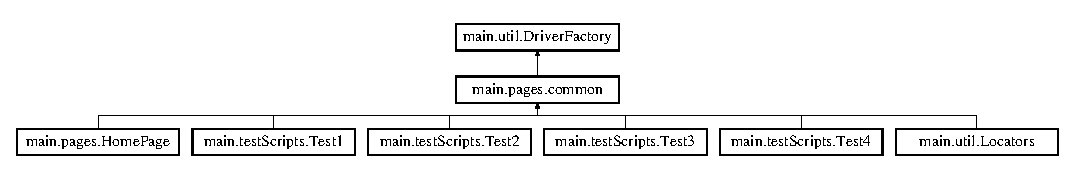
\includegraphics[height=1.866667cm]{classmain_1_1pages_1_1common}
\end{center}
\end{figure}
\subsection*{Public Member Functions}
\begin{DoxyCompactItemize}
\item 
void \mbox{\hyperlink{classmain_1_1pages_1_1common_aedb8bb00674efe1e7b551e14d10219ba}{start\+Test\+Environment}} (String test\+Case\+Name, String browser\+Type)
\item 
void \mbox{\hyperlink{classmain_1_1pages_1_1common_a04df2281dc9f8ea63ba88528030c54c2}{close\+Test\+Environment}} (String test\+Case\+Name)
\item 
void \mbox{\hyperlink{classmain_1_1pages_1_1common_a7b9ae10e9d8cfb4504c06dc25d133c1f}{take\+Screen\+Shot}} (String name\+Of\+Screen\+Shot)
\end{DoxyCompactItemize}
\subsection*{Static Public Member Functions}
\begin{DoxyCompactItemize}
\item 
static boolean \mbox{\hyperlink{classmain_1_1pages_1_1common_aa1116271e95e4d544eab6c38d160a1ab}{is64\+Bit\+System}} ()
\item 
static String \mbox{\hyperlink{classmain_1_1pages_1_1common_a75bf8538e39f1ea3759eebeef9edfa22}{is\+Link\+Broken}} (U\+RL url)  throws Exception 	 
\end{DoxyCompactItemize}
\subsection*{Static Public Attributes}
\begin{DoxyCompactItemize}
\item 
\mbox{\Hypertarget{classmain_1_1pages_1_1common_a3769216efb920a003c2bb86ad9cee902}\label{classmain_1_1pages_1_1common_a3769216efb920a003c2bb86ad9cee902}} 
static boolean {\bfseries test\+Status} = true
\item 
\mbox{\Hypertarget{classmain_1_1pages_1_1common_a3061c243240e93e69ddd669f66d40d25}\label{classmain_1_1pages_1_1common_a3061c243240e93e69ddd669f66d40d25}} 
static Soft\+Assert {\bfseries soft\+Assert}
\item 
\mbox{\Hypertarget{classmain_1_1pages_1_1common_a5a1d1b1d4a665cb359580db45574cd62}\label{classmain_1_1pages_1_1common_a5a1d1b1d4a665cb359580db45574cd62}} 
static \mbox{\hyperlink{classmain_1_1util_1_1_log___handler}{Log\+\_\+\+Handler}} {\bfseries log\+\_\+\+Handler}
\item 
\mbox{\Hypertarget{classmain_1_1pages_1_1common_a20a15df6732341b69f37947f111c38ab}\label{classmain_1_1pages_1_1common_a20a15df6732341b69f37947f111c38ab}} 
static int {\bfseries test\+Screen\+Shot\+Seriel}
\end{DoxyCompactItemize}


\subsection{Detailed Description}
Provided for initializing all the common methods across Open\+Weather project. 

\subsection{Member Function Documentation}
\mbox{\Hypertarget{classmain_1_1pages_1_1common_a04df2281dc9f8ea63ba88528030c54c2}\label{classmain_1_1pages_1_1common_a04df2281dc9f8ea63ba88528030c54c2}} 
\index{main\+::pages\+::common@{main\+::pages\+::common}!close\+Test\+Environment@{close\+Test\+Environment}}
\index{close\+Test\+Environment@{close\+Test\+Environment}!main\+::pages\+::common@{main\+::pages\+::common}}
\subsubsection{\texorpdfstring{close\+Test\+Environment()}{closeTestEnvironment()}}
{\footnotesize\ttfamily void main.\+pages.\+common.\+close\+Test\+Environment (\begin{DoxyParamCaption}\item[{String}]{test\+Case\+Name }\end{DoxyParamCaption})}

Common methods to close Test environment. 
\begin{DoxyParams}{Parameters}
{\em test\+Case\+Name} & \\
\hline
\end{DoxyParams}
\begin{DoxyReturn}{Returns}
void 
\end{DoxyReturn}
\mbox{\Hypertarget{classmain_1_1pages_1_1common_aa1116271e95e4d544eab6c38d160a1ab}\label{classmain_1_1pages_1_1common_aa1116271e95e4d544eab6c38d160a1ab}} 
\index{main\+::pages\+::common@{main\+::pages\+::common}!is64\+Bit\+System@{is64\+Bit\+System}}
\index{is64\+Bit\+System@{is64\+Bit\+System}!main\+::pages\+::common@{main\+::pages\+::common}}
\subsubsection{\texorpdfstring{is64\+Bit\+System()}{is64BitSystem()}}
{\footnotesize\ttfamily static boolean main.\+pages.\+common.\+is64\+Bit\+System (\begin{DoxyParamCaption}{ }\end{DoxyParamCaption})\hspace{0.3cm}{\ttfamily [static]}}

Common methods to identify the systems\textquotesingle{} bit version on bases of Sselenium Driver version passes to script. \begin{DoxyReturn}{Returns}
void 
\end{DoxyReturn}
\mbox{\Hypertarget{classmain_1_1pages_1_1common_a75bf8538e39f1ea3759eebeef9edfa22}\label{classmain_1_1pages_1_1common_a75bf8538e39f1ea3759eebeef9edfa22}} 
\index{main\+::pages\+::common@{main\+::pages\+::common}!is\+Link\+Broken@{is\+Link\+Broken}}
\index{is\+Link\+Broken@{is\+Link\+Broken}!main\+::pages\+::common@{main\+::pages\+::common}}
\subsubsection{\texorpdfstring{is\+Link\+Broken()}{isLinkBroken()}}
{\footnotesize\ttfamily static String main.\+pages.\+common.\+is\+Link\+Broken (\begin{DoxyParamCaption}\item[{U\+RL}]{url }\end{DoxyParamCaption}) throws Exception\hspace{0.3cm}{\ttfamily [static]}}

Common methods to identify if the link available on webpage is broken. 
\begin{DoxyParams}{Parameters}
{\em url} & of the link \\
\hline
\end{DoxyParams}
\begin{DoxyReturn}{Returns}
string 
\end{DoxyReturn}
\mbox{\Hypertarget{classmain_1_1pages_1_1common_aedb8bb00674efe1e7b551e14d10219ba}\label{classmain_1_1pages_1_1common_aedb8bb00674efe1e7b551e14d10219ba}} 
\index{main\+::pages\+::common@{main\+::pages\+::common}!start\+Test\+Environment@{start\+Test\+Environment}}
\index{start\+Test\+Environment@{start\+Test\+Environment}!main\+::pages\+::common@{main\+::pages\+::common}}
\subsubsection{\texorpdfstring{start\+Test\+Environment()}{startTestEnvironment()}}
{\footnotesize\ttfamily void main.\+pages.\+common.\+start\+Test\+Environment (\begin{DoxyParamCaption}\item[{String}]{test\+Case\+Name,  }\item[{String}]{browser\+Type }\end{DoxyParamCaption})}

A common method to Start of Test environment. 
\begin{DoxyParams}{Parameters}
{\em test\+Case\+Name,browser\+Type} & \\
\hline
\end{DoxyParams}
\begin{DoxyReturn}{Returns}
void 
\end{DoxyReturn}
\mbox{\Hypertarget{classmain_1_1pages_1_1common_a7b9ae10e9d8cfb4504c06dc25d133c1f}\label{classmain_1_1pages_1_1common_a7b9ae10e9d8cfb4504c06dc25d133c1f}} 
\index{main\+::pages\+::common@{main\+::pages\+::common}!take\+Screen\+Shot@{take\+Screen\+Shot}}
\index{take\+Screen\+Shot@{take\+Screen\+Shot}!main\+::pages\+::common@{main\+::pages\+::common}}
\subsubsection{\texorpdfstring{take\+Screen\+Shot()}{takeScreenShot()}}
{\footnotesize\ttfamily void main.\+pages.\+common.\+take\+Screen\+Shot (\begin{DoxyParamCaption}\item[{String}]{name\+Of\+Screen\+Shot }\end{DoxyParamCaption})}

Common methods to Take screenshot per failure during test execution. 
\begin{DoxyParams}{Parameters}
{\em name\+Of\+Screen\+Shot} & \\
\hline
\end{DoxyParams}
\begin{DoxyReturn}{Returns}
void 
\end{DoxyReturn}


The documentation for this class was generated from the following file\+:\begin{DoxyCompactItemize}
\item 
main/pages/common.\+java\end{DoxyCompactItemize}

\hypertarget{classmain_1_1util_1_1_driver_factory}{}\section{main.\+util.\+Driver\+Factory Class Reference}
\label{classmain_1_1util_1_1_driver_factory}\index{main.\+util.\+Driver\+Factory@{main.\+util.\+Driver\+Factory}}
Inheritance diagram for main.\+util.\+Driver\+Factory\+:\begin{figure}[H]
\begin{center}
\leavevmode
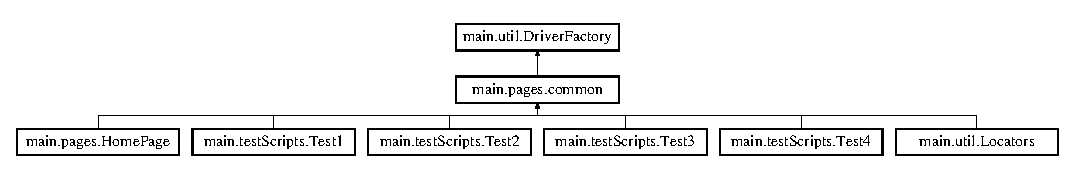
\includegraphics[height=1.866667cm]{classmain_1_1util_1_1_driver_factory}
\end{center}
\end{figure}
\subsection*{Static Public Member Functions}
\begin{DoxyCompactItemize}
\item 
static void \mbox{\hyperlink{classmain_1_1util_1_1_driver_factory_a0e334a84a12fdd821fc19df6bb29241e}{initialize\+Driver}} (String browser\+Type)
\item 
static void \mbox{\hyperlink{classmain_1_1util_1_1_driver_factory_abdd3d0a38b3fa5faa46119170c124518}{stop\+Driver}} ()
\item 
static void \mbox{\hyperlink{classmain_1_1util_1_1_driver_factory_a8e5bfb00afc1564bf60ec2491953ad42}{quit\+Driver}} ()
\item 
static String \mbox{\hyperlink{classmain_1_1util_1_1_driver_factory_a31b83afd40c9f0a7d24661ccbce90d83}{get\+Current\+Folder\+Path}} ()
\end{DoxyCompactItemize}
\subsection*{Static Public Attributes}
\begin{DoxyCompactItemize}
\item 
\mbox{\Hypertarget{classmain_1_1util_1_1_driver_factory_a8afca6d6beb8c3486a6fd673d19ea79b}\label{classmain_1_1util_1_1_driver_factory_a8afca6d6beb8c3486a6fd673d19ea79b}} 
static Web\+Driver {\bfseries app\+Driver}
\end{DoxyCompactItemize}


\subsection{Member Function Documentation}
\mbox{\Hypertarget{classmain_1_1util_1_1_driver_factory_a31b83afd40c9f0a7d24661ccbce90d83}\label{classmain_1_1util_1_1_driver_factory_a31b83afd40c9f0a7d24661ccbce90d83}} 
\index{main\+::util\+::\+Driver\+Factory@{main\+::util\+::\+Driver\+Factory}!get\+Current\+Folder\+Path@{get\+Current\+Folder\+Path}}
\index{get\+Current\+Folder\+Path@{get\+Current\+Folder\+Path}!main\+::util\+::\+Driver\+Factory@{main\+::util\+::\+Driver\+Factory}}
\subsubsection{\texorpdfstring{get\+Current\+Folder\+Path()}{getCurrentFolderPath()}}
{\footnotesize\ttfamily static String main.\+util.\+Driver\+Factory.\+get\+Current\+Folder\+Path (\begin{DoxyParamCaption}{ }\end{DoxyParamCaption})\hspace{0.3cm}{\ttfamily [static]}}

A static method to get the current folder path. \begin{DoxyReturn}{Returns}
void 
\end{DoxyReturn}
\mbox{\Hypertarget{classmain_1_1util_1_1_driver_factory_a0e334a84a12fdd821fc19df6bb29241e}\label{classmain_1_1util_1_1_driver_factory_a0e334a84a12fdd821fc19df6bb29241e}} 
\index{main\+::util\+::\+Driver\+Factory@{main\+::util\+::\+Driver\+Factory}!initialize\+Driver@{initialize\+Driver}}
\index{initialize\+Driver@{initialize\+Driver}!main\+::util\+::\+Driver\+Factory@{main\+::util\+::\+Driver\+Factory}}
\subsubsection{\texorpdfstring{initialize\+Driver()}{initializeDriver()}}
{\footnotesize\ttfamily static void main.\+util.\+Driver\+Factory.\+initialize\+Driver (\begin{DoxyParamCaption}\item[{String}]{browser\+Type }\end{DoxyParamCaption})\hspace{0.3cm}{\ttfamily [static]}}

A static method to initialize the webdriver as per given browser type. \begin{DoxyReturn}{Returns}
void 
\end{DoxyReturn}
\mbox{\Hypertarget{classmain_1_1util_1_1_driver_factory_a8e5bfb00afc1564bf60ec2491953ad42}\label{classmain_1_1util_1_1_driver_factory_a8e5bfb00afc1564bf60ec2491953ad42}} 
\index{main\+::util\+::\+Driver\+Factory@{main\+::util\+::\+Driver\+Factory}!quit\+Driver@{quit\+Driver}}
\index{quit\+Driver@{quit\+Driver}!main\+::util\+::\+Driver\+Factory@{main\+::util\+::\+Driver\+Factory}}
\subsubsection{\texorpdfstring{quit\+Driver()}{quitDriver()}}
{\footnotesize\ttfamily static void main.\+util.\+Driver\+Factory.\+quit\+Driver (\begin{DoxyParamCaption}{ }\end{DoxyParamCaption})\hspace{0.3cm}{\ttfamily [static]}}

A static method to quit the webdriver. \begin{DoxyReturn}{Returns}
void 
\end{DoxyReturn}
\mbox{\Hypertarget{classmain_1_1util_1_1_driver_factory_abdd3d0a38b3fa5faa46119170c124518}\label{classmain_1_1util_1_1_driver_factory_abdd3d0a38b3fa5faa46119170c124518}} 
\index{main\+::util\+::\+Driver\+Factory@{main\+::util\+::\+Driver\+Factory}!stop\+Driver@{stop\+Driver}}
\index{stop\+Driver@{stop\+Driver}!main\+::util\+::\+Driver\+Factory@{main\+::util\+::\+Driver\+Factory}}
\subsubsection{\texorpdfstring{stop\+Driver()}{stopDriver()}}
{\footnotesize\ttfamily static void main.\+util.\+Driver\+Factory.\+stop\+Driver (\begin{DoxyParamCaption}{ }\end{DoxyParamCaption})\hspace{0.3cm}{\ttfamily [static]}}

A static method to stop the webdriver. \begin{DoxyReturn}{Returns}
void 
\end{DoxyReturn}


The documentation for this class was generated from the following file\+:\begin{DoxyCompactItemize}
\item 
main/util/Driver\+Factory.\+java\end{DoxyCompactItemize}

\hypertarget{classmain_1_1util_1_1_framework_constants}{}\section{main.\+util.\+Framework\+Constants Class Reference}
\label{classmain_1_1util_1_1_framework_constants}\index{main.\+util.\+Framework\+Constants@{main.\+util.\+Framework\+Constants}}
\subsection*{Static Public Attributes}
\begin{DoxyCompactItemize}
\item 
\mbox{\Hypertarget{classmain_1_1util_1_1_framework_constants_aec4e078646cebcd7f5730916bbcb7261}\label{classmain_1_1util_1_1_framework_constants_aec4e078646cebcd7f5730916bbcb7261}} 
static final String {\bfseries D\+R\+I\+V\+E\+R\+\_\+\+T\+Y\+PE} = \char`\"{}Chrome\char`\"{}
\item 
\mbox{\Hypertarget{classmain_1_1util_1_1_framework_constants_a883117dd023b6a5f005151f6bcfc7d48}\label{classmain_1_1util_1_1_framework_constants_a883117dd023b6a5f005151f6bcfc7d48}} 
static final String {\bfseries C\+H\+R\+O\+M\+E\+\_\+\+D\+R\+I\+V\+E\+R\+E\+X\+E\+\_\+\+P\+A\+TH} = \char`\"{}.\textbackslash{}\textbackslash{}src\textbackslash{}\textbackslash{}test\textbackslash{}\textbackslash{}resources\textbackslash{}\textbackslash{}\+Drivers\textbackslash{}\textbackslash{}chromedriver\+\_\+32.\+exe\char`\"{}
\item 
\mbox{\Hypertarget{classmain_1_1util_1_1_framework_constants_a977fc0daaebe258859a930c0148d245c}\label{classmain_1_1util_1_1_framework_constants_a977fc0daaebe258859a930c0148d245c}} 
static final String {\bfseries G\+E\+C\+K\+O\+\_\+32\+\_\+\+D\+R\+I\+V\+E\+R\+E\+X\+E\+\_\+\+P\+A\+TH} = \char`\"{}.\textbackslash{}\textbackslash{}src\textbackslash{}\textbackslash{}test\textbackslash{}\textbackslash{}resources\textbackslash{}\textbackslash{}\+Drivers\textbackslash{}\textbackslash{}geckodriver\+\_\+32.\+exe\char`\"{}
\item 
\mbox{\Hypertarget{classmain_1_1util_1_1_framework_constants_a7e1645c395a392629e671eb24855680c}\label{classmain_1_1util_1_1_framework_constants_a7e1645c395a392629e671eb24855680c}} 
static final String {\bfseries G\+E\+C\+K\+O\+\_\+64\+\_\+\+D\+R\+I\+V\+E\+R\+E\+X\+E\+\_\+\+P\+A\+TH} = \char`\"{}.\textbackslash{}\textbackslash{}src\textbackslash{}\textbackslash{}test\textbackslash{}\textbackslash{}resources\textbackslash{}\textbackslash{}\+Drivers\textbackslash{}\textbackslash{}geckodriver\+\_\+64.\+exe\char`\"{}
\item 
\mbox{\Hypertarget{classmain_1_1util_1_1_framework_constants_a806a1e26fc762fef157bb3028212603b}\label{classmain_1_1util_1_1_framework_constants_a806a1e26fc762fef157bb3028212603b}} 
static final String {\bfseries I\+E\+\_\+32\+\_\+\+D\+R\+I\+V\+E\+R\+E\+X\+E\+\_\+\+P\+A\+TH} = \char`\"{}.\textbackslash{}\textbackslash{}src\textbackslash{}\textbackslash{}test\textbackslash{}\textbackslash{}resources\textbackslash{}\textbackslash{}\+Drivers\textbackslash{}\textbackslash{}\+I\+E\+Driver\+Server\+\_\+32.\+exe\char`\"{}
\item 
\mbox{\Hypertarget{classmain_1_1util_1_1_framework_constants_aa8f9c7c60030a03a6c4c992be414f2a5}\label{classmain_1_1util_1_1_framework_constants_aa8f9c7c60030a03a6c4c992be414f2a5}} 
static final String {\bfseries I\+E\+\_\+64\+\_\+\+D\+R\+I\+V\+E\+R\+E\+X\+E\+\_\+\+P\+A\+TH} = \char`\"{}.\textbackslash{}\textbackslash{}src\textbackslash{}\textbackslash{}test\textbackslash{}\textbackslash{}resources\textbackslash{}\textbackslash{}\+Drivers\textbackslash{}\textbackslash{}\+I\+E\+Driver\+Server\+\_\+64.\+exe\char`\"{}
\item 
\mbox{\Hypertarget{classmain_1_1util_1_1_framework_constants_a7069c6bc1634ca068b167fc62717640b}\label{classmain_1_1util_1_1_framework_constants_a7069c6bc1634ca068b167fc62717640b}} 
static final String {\bfseries A\+P\+P\+\_\+\+U\+RL} = \char`\"{}https\+://openweathermap.\+org\char`\"{}
\item 
\mbox{\Hypertarget{classmain_1_1util_1_1_framework_constants_a77eb73cf58cc42747c7ea34d2489242c}\label{classmain_1_1util_1_1_framework_constants_a77eb73cf58cc42747c7ea34d2489242c}} 
static final String {\bfseries W\+O\+R\+K\+I\+N\+G\+\_\+\+D\+IR} = \char`\"{}..\char`\"{}
\item 
\mbox{\Hypertarget{classmain_1_1util_1_1_framework_constants_a500fed0f1ec588999c097ffee7390868}\label{classmain_1_1util_1_1_framework_constants_a500fed0f1ec588999c097ffee7390868}} 
static final String {\bfseries R\+E\+S\+O\+U\+R\+C\+E\+S\+\_\+\+F\+O\+L\+D\+ER} = \char`\"{}.\textbackslash{}\textbackslash{}src\textbackslash{}\textbackslash{}test\textbackslash{}\textbackslash{}resources\textbackslash{}\textbackslash{}\char`\"{}
\item 
\mbox{\Hypertarget{classmain_1_1util_1_1_framework_constants_ab50a2ad5c33ae063332c66d934e3c5be}\label{classmain_1_1util_1_1_framework_constants_ab50a2ad5c33ae063332c66d934e3c5be}} 
static final String {\bfseries R\+E\+S\+O\+U\+R\+C\+E\+S\+\_\+\+L\+O\+C\+A\+T\+OR} = \char`\"{}.\textbackslash{}\textbackslash{}src\textbackslash{}\textbackslash{}test\textbackslash{}\textbackslash{}resources\textbackslash{}\textbackslash{}\+Locators\textbackslash{}\textbackslash{}\char`\"{}
\item 
\mbox{\Hypertarget{classmain_1_1util_1_1_framework_constants_a7b8e916dd0e23b7c49c0c33966c18743}\label{classmain_1_1util_1_1_framework_constants_a7b8e916dd0e23b7c49c0c33966c18743}} 
static final String {\bfseries C\+H\+R\+O\+M\+E\+\_\+\+E\+X\+T\+E\+N\+S\+I\+O\+N\+\_\+\+F\+O\+L\+D\+ER} = \char`\"{}/chrome-\/extensions\char`\"{}
\item 
\mbox{\Hypertarget{classmain_1_1util_1_1_framework_constants_a40c286eea9534c84a3edc4f6dcf24be0}\label{classmain_1_1util_1_1_framework_constants_a40c286eea9534c84a3edc4f6dcf24be0}} 
static final String {\bfseries L\+O\+G4\+J\+P\+R\+O\+P\+E\+R\+T\+Y\+F\+I\+L\+E\+L\+OC} = \char`\"{}.\textbackslash{}\textbackslash{}src\textbackslash{}\textbackslash{}test\textbackslash{}\textbackslash{}resources\textbackslash{}\textbackslash{}\+Drivers\textbackslash{}\textbackslash{}log4j.\+properties\char`\"{}
\item 
\mbox{\Hypertarget{classmain_1_1util_1_1_framework_constants_aa5f8d30ec17c454473052f96f5204549}\label{classmain_1_1util_1_1_framework_constants_aa5f8d30ec17c454473052f96f5204549}} 
static final String {\bfseries L\+O\+G\+F\+I\+L\+E\+L\+OC} = \char`\"{}.\textbackslash{}\textbackslash{}logs\textbackslash{}\textbackslash{}\+Logger.\+log\char`\"{}
\item 
\mbox{\Hypertarget{classmain_1_1util_1_1_framework_constants_abfc9634deff385aea74a4d30efbbe6fd}\label{classmain_1_1util_1_1_framework_constants_abfc9634deff385aea74a4d30efbbe6fd}} 
static final String {\bfseries L\+O\+G\+F\+I\+L\+E\+B\+A\+C\+K\+U\+P\+L\+OC} = \char`\"{}.\textbackslash{}\textbackslash{}logs\textbackslash{}\textbackslash{}\+Log\+Backup\char`\"{}
\item 
\mbox{\Hypertarget{classmain_1_1util_1_1_framework_constants_ae14f36d897208826e889a2b7cc8726d4}\label{classmain_1_1util_1_1_framework_constants_ae14f36d897208826e889a2b7cc8726d4}} 
static final String {\bfseries E\+R\+R\+O\+R\+S\+C\+R\+E\+E\+N\+S\+H\+O\+T\+L\+OC} = \char`\"{}.\textbackslash{}\textbackslash{}logs\textbackslash{}\textbackslash{}\+Screen\+Shots\char`\"{}
\end{DoxyCompactItemize}


\subsection{Detailed Description}
A class to provide the path of necessary repository and paths. Making these as final to have them set only once. 

The documentation for this class was generated from the following file\+:\begin{DoxyCompactItemize}
\item 
main/util/Framework\+Constants.\+java\end{DoxyCompactItemize}

\hypertarget{classmain_1_1pages_1_1_home_page}{}\section{main.\+pages.\+Home\+Page Class Reference}
\label{classmain_1_1pages_1_1_home_page}\index{main.\+pages.\+Home\+Page@{main.\+pages.\+Home\+Page}}
Inheritance diagram for main.\+pages.\+Home\+Page\+:\begin{figure}[H]
\begin{center}
\leavevmode
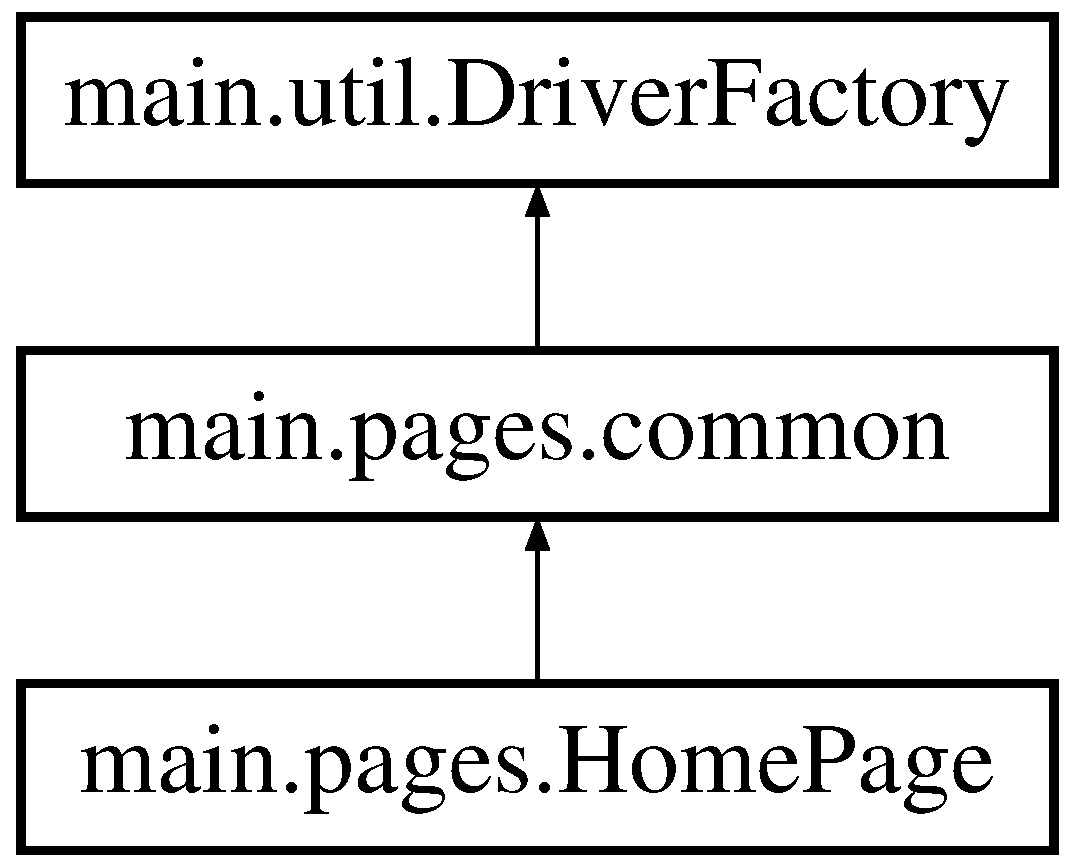
\includegraphics[height=3.000000cm]{classmain_1_1pages_1_1_home_page}
\end{center}
\end{figure}
\subsection*{Public Member Functions}
\begin{DoxyCompactItemize}
\item 
\mbox{\hyperlink{classmain_1_1pages_1_1_home_page_a7fb96c9279ead0bb1905390008df332b}{Home\+Page}} ()
\item 
\mbox{\Hypertarget{classmain_1_1pages_1_1_home_page_a488bb73f12e82d543ad669398851b698}\label{classmain_1_1pages_1_1_home_page_a488bb73f12e82d543ad669398851b698}} 
By {\bfseries Search\+Specific\+Result\+To\+User\+Data} (String user\+Data)
\item 
boolean \mbox{\hyperlink{classmain_1_1pages_1_1_home_page_ab12db71ec89778964fe831fdbc8f78d2}{verify\+Home\+Page\+Elements}} ()
\item 
boolean \mbox{\hyperlink{classmain_1_1pages_1_1_home_page_a4ea73ab43b733f85412185481f7cfbe5}{search\+Text\+In\+Search\+Box}} (String search\+Text)
\item 
boolean \mbox{\hyperlink{classmain_1_1pages_1_1_home_page_a23f149b5230539d36088c9d85ddd6fa7}{verify\+Search\+Result\+Dislayed}} (String search\+Text)
\item 
boolean \mbox{\hyperlink{classmain_1_1pages_1_1_home_page_a08b21c4d5923e0fc37c258ed4b854f37}{verify\+Search\+Result\+Not\+Dislayed}} ()
\end{DoxyCompactItemize}
\subsection*{Additional Inherited Members}


\subsection{Detailed Description}
\begin{DoxyAuthor}{Author}
rawatp1 
\end{DoxyAuthor}


\subsection{Constructor \& Destructor Documentation}
\mbox{\Hypertarget{classmain_1_1pages_1_1_home_page_a7fb96c9279ead0bb1905390008df332b}\label{classmain_1_1pages_1_1_home_page_a7fb96c9279ead0bb1905390008df332b}} 
\index{main\+::pages\+::\+Home\+Page@{main\+::pages\+::\+Home\+Page}!Home\+Page@{Home\+Page}}
\index{Home\+Page@{Home\+Page}!main\+::pages\+::\+Home\+Page@{main\+::pages\+::\+Home\+Page}}
\subsubsection{\texorpdfstring{Home\+Page()}{HomePage()}}
{\footnotesize\ttfamily main.\+pages.\+Home\+Page.\+Home\+Page (\begin{DoxyParamCaption}{ }\end{DoxyParamCaption})}

Constructor to identify the browser type property as locators could be different as per a web browser. 

\subsection{Member Function Documentation}
\mbox{\Hypertarget{classmain_1_1pages_1_1_home_page_a4ea73ab43b733f85412185481f7cfbe5}\label{classmain_1_1pages_1_1_home_page_a4ea73ab43b733f85412185481f7cfbe5}} 
\index{main\+::pages\+::\+Home\+Page@{main\+::pages\+::\+Home\+Page}!search\+Text\+In\+Search\+Box@{search\+Text\+In\+Search\+Box}}
\index{search\+Text\+In\+Search\+Box@{search\+Text\+In\+Search\+Box}!main\+::pages\+::\+Home\+Page@{main\+::pages\+::\+Home\+Page}}
\subsubsection{\texorpdfstring{search\+Text\+In\+Search\+Box()}{searchTextInSearchBox()}}
{\footnotesize\ttfamily boolean main.\+pages.\+Home\+Page.\+search\+Text\+In\+Search\+Box (\begin{DoxyParamCaption}\item[{String}]{search\+Text }\end{DoxyParamCaption})}

A methods to enter search text in search box of home page. 
\begin{DoxyParams}{Parameters}
{\em search\+Text} & \\
\hline
\end{DoxyParams}
\begin{DoxyReturn}{Returns}
boolean 
\end{DoxyReturn}
\mbox{\Hypertarget{classmain_1_1pages_1_1_home_page_ab12db71ec89778964fe831fdbc8f78d2}\label{classmain_1_1pages_1_1_home_page_ab12db71ec89778964fe831fdbc8f78d2}} 
\index{main\+::pages\+::\+Home\+Page@{main\+::pages\+::\+Home\+Page}!verify\+Home\+Page\+Elements@{verify\+Home\+Page\+Elements}}
\index{verify\+Home\+Page\+Elements@{verify\+Home\+Page\+Elements}!main\+::pages\+::\+Home\+Page@{main\+::pages\+::\+Home\+Page}}
\subsubsection{\texorpdfstring{verify\+Home\+Page\+Elements()}{verifyHomePageElements()}}
{\footnotesize\ttfamily boolean main.\+pages.\+Home\+Page.\+verify\+Home\+Page\+Elements (\begin{DoxyParamCaption}{ }\end{DoxyParamCaption})}

A methods to verify Home page elements. \begin{DoxyReturn}{Returns}
boolean 
\end{DoxyReturn}
\mbox{\Hypertarget{classmain_1_1pages_1_1_home_page_a23f149b5230539d36088c9d85ddd6fa7}\label{classmain_1_1pages_1_1_home_page_a23f149b5230539d36088c9d85ddd6fa7}} 
\index{main\+::pages\+::\+Home\+Page@{main\+::pages\+::\+Home\+Page}!verify\+Search\+Result\+Dislayed@{verify\+Search\+Result\+Dislayed}}
\index{verify\+Search\+Result\+Dislayed@{verify\+Search\+Result\+Dislayed}!main\+::pages\+::\+Home\+Page@{main\+::pages\+::\+Home\+Page}}
\subsubsection{\texorpdfstring{verify\+Search\+Result\+Dislayed()}{verifySearchResultDislayed()}}
{\footnotesize\ttfamily boolean main.\+pages.\+Home\+Page.\+verify\+Search\+Result\+Dislayed (\begin{DoxyParamCaption}\item[{String}]{search\+Text }\end{DoxyParamCaption})}

A methods to verify if the search result is displayed post given a search. 
\begin{DoxyParams}{Parameters}
{\em search\+Text} & \\
\hline
\end{DoxyParams}
\begin{DoxyReturn}{Returns}
boolean 
\end{DoxyReturn}
\mbox{\Hypertarget{classmain_1_1pages_1_1_home_page_a08b21c4d5923e0fc37c258ed4b854f37}\label{classmain_1_1pages_1_1_home_page_a08b21c4d5923e0fc37c258ed4b854f37}} 
\index{main\+::pages\+::\+Home\+Page@{main\+::pages\+::\+Home\+Page}!verify\+Search\+Result\+Not\+Dislayed@{verify\+Search\+Result\+Not\+Dislayed}}
\index{verify\+Search\+Result\+Not\+Dislayed@{verify\+Search\+Result\+Not\+Dislayed}!main\+::pages\+::\+Home\+Page@{main\+::pages\+::\+Home\+Page}}
\subsubsection{\texorpdfstring{verify\+Search\+Result\+Not\+Dislayed()}{verifySearchResultNotDislayed()}}
{\footnotesize\ttfamily boolean main.\+pages.\+Home\+Page.\+verify\+Search\+Result\+Not\+Dislayed (\begin{DoxyParamCaption}{ }\end{DoxyParamCaption})}

A methods to verify that the search result should not be displayed if a invalid city name given to search. \begin{DoxyReturn}{Returns}
boolean 
\end{DoxyReturn}


The documentation for this class was generated from the following file\+:\begin{DoxyCompactItemize}
\item 
main/pages/Home\+Page.\+java\end{DoxyCompactItemize}

\hypertarget{classmain_1_1util_1_1_locators}{}\section{main.\+util.\+Locators Class Reference}
\label{classmain_1_1util_1_1_locators}\index{main.\+util.\+Locators@{main.\+util.\+Locators}}
Inheritance diagram for main.\+util.\+Locators\+:\begin{figure}[H]
\begin{center}
\leavevmode
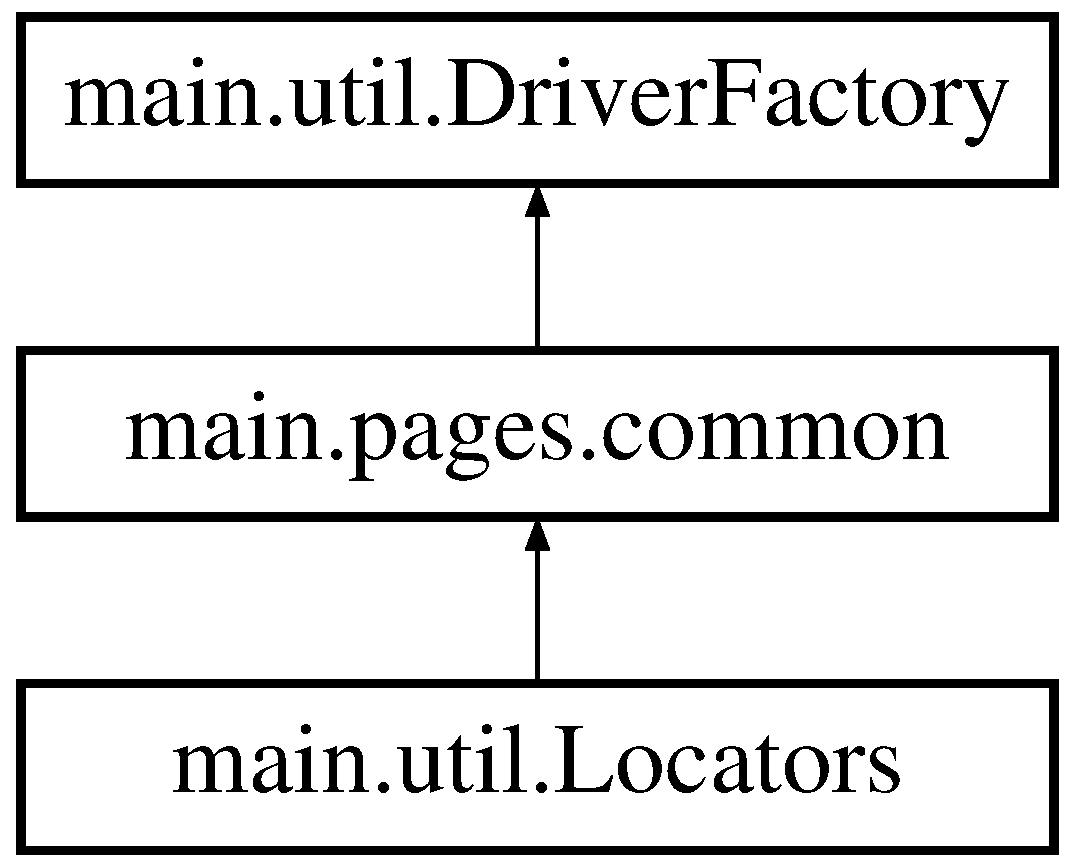
\includegraphics[height=3.000000cm]{classmain_1_1util_1_1_locators}
\end{center}
\end{figure}
\subsection*{Static Public Member Functions}
\begin{DoxyCompactItemize}
\item 
static By \mbox{\hyperlink{classmain_1_1util_1_1_locators_abfccf35b881fdba5d096dfed34153a7e}{get\+By}} (String key, String path)
\item 
static By \mbox{\hyperlink{classmain_1_1util_1_1_locators_a1c63d6c289e5b1f5f4b0a399cf6d20b6}{get\+By}} (String key, String path, String userdata)
\item 
static By \mbox{\hyperlink{classmain_1_1util_1_1_locators_a2aff991dbee052ae04c110eaa6a94686}{by\+Xpath\+Span\+Text}} (String text)
\item 
static By \mbox{\hyperlink{classmain_1_1util_1_1_locators_a8c86ef6c524f7ec696db7f81d6243211}{by\+Xpath\+Span\+Text\+Contains}} (String text)
\item 
static By \mbox{\hyperlink{classmain_1_1util_1_1_locators_a19c55393acbfebff041901aa2917d489}{by\+Partial\+Link\+Text}} (String text)
\end{DoxyCompactItemize}
\subsection*{Additional Inherited Members}


\subsection{Detailed Description}
Provided for Identifying the locators on bases of Dynamic web elements identification, so there is no need to hardcode of \mbox{\hyperlink{classmain_1_1util_1_1_locators}{Locators}}. 

\subsection{Member Function Documentation}
\mbox{\Hypertarget{classmain_1_1util_1_1_locators_a19c55393acbfebff041901aa2917d489}\label{classmain_1_1util_1_1_locators_a19c55393acbfebff041901aa2917d489}} 
\index{main\+::util\+::\+Locators@{main\+::util\+::\+Locators}!by\+Partial\+Link\+Text@{by\+Partial\+Link\+Text}}
\index{by\+Partial\+Link\+Text@{by\+Partial\+Link\+Text}!main\+::util\+::\+Locators@{main\+::util\+::\+Locators}}
\subsubsection{\texorpdfstring{by\+Partial\+Link\+Text()}{byPartialLinkText()}}
{\footnotesize\ttfamily static By main.\+util.\+Locators.\+by\+Partial\+Link\+Text (\begin{DoxyParamCaption}\item[{String}]{text }\end{DoxyParamCaption})\hspace{0.3cm}{\ttfamily [static]}}

A static method to read the locator values on basis of partial link text 
\begin{DoxyParams}{Parameters}
{\em input} & text as span on basis of partial link text \\
\hline
\end{DoxyParams}
\begin{DoxyReturn}{Returns}
By 
\end{DoxyReturn}
\mbox{\Hypertarget{classmain_1_1util_1_1_locators_a2aff991dbee052ae04c110eaa6a94686}\label{classmain_1_1util_1_1_locators_a2aff991dbee052ae04c110eaa6a94686}} 
\index{main\+::util\+::\+Locators@{main\+::util\+::\+Locators}!by\+Xpath\+Span\+Text@{by\+Xpath\+Span\+Text}}
\index{by\+Xpath\+Span\+Text@{by\+Xpath\+Span\+Text}!main\+::util\+::\+Locators@{main\+::util\+::\+Locators}}
\subsubsection{\texorpdfstring{by\+Xpath\+Span\+Text()}{byXpathSpanText()}}
{\footnotesize\ttfamily static By main.\+util.\+Locators.\+by\+Xpath\+Span\+Text (\begin{DoxyParamCaption}\item[{String}]{text }\end{DoxyParamCaption})\hspace{0.3cm}{\ttfamily [static]}}

A static method to read the locator values on basis of span text 
\begin{DoxyParams}{Parameters}
{\em input} & text as span \\
\hline
\end{DoxyParams}
\begin{DoxyReturn}{Returns}
By 
\end{DoxyReturn}
\mbox{\Hypertarget{classmain_1_1util_1_1_locators_a8c86ef6c524f7ec696db7f81d6243211}\label{classmain_1_1util_1_1_locators_a8c86ef6c524f7ec696db7f81d6243211}} 
\index{main\+::util\+::\+Locators@{main\+::util\+::\+Locators}!by\+Xpath\+Span\+Text\+Contains@{by\+Xpath\+Span\+Text\+Contains}}
\index{by\+Xpath\+Span\+Text\+Contains@{by\+Xpath\+Span\+Text\+Contains}!main\+::util\+::\+Locators@{main\+::util\+::\+Locators}}
\subsubsection{\texorpdfstring{by\+Xpath\+Span\+Text\+Contains()}{byXpathSpanTextContains()}}
{\footnotesize\ttfamily static By main.\+util.\+Locators.\+by\+Xpath\+Span\+Text\+Contains (\begin{DoxyParamCaption}\item[{String}]{text }\end{DoxyParamCaption})\hspace{0.3cm}{\ttfamily [static]}}

A static method to read the locator values on basis of span text contains 
\begin{DoxyParams}{Parameters}
{\em input} & text as span on basis of partial check \\
\hline
\end{DoxyParams}
\begin{DoxyReturn}{Returns}
By 
\end{DoxyReturn}
\mbox{\Hypertarget{classmain_1_1util_1_1_locators_abfccf35b881fdba5d096dfed34153a7e}\label{classmain_1_1util_1_1_locators_abfccf35b881fdba5d096dfed34153a7e}} 
\index{main\+::util\+::\+Locators@{main\+::util\+::\+Locators}!get\+By@{get\+By}}
\index{get\+By@{get\+By}!main\+::util\+::\+Locators@{main\+::util\+::\+Locators}}
\subsubsection{\texorpdfstring{get\+By()}{getBy()}\hspace{0.1cm}{\footnotesize\ttfamily [1/2]}}
{\footnotesize\ttfamily static By main.\+util.\+Locators.\+get\+By (\begin{DoxyParamCaption}\item[{String}]{key,  }\item[{String}]{path }\end{DoxyParamCaption})\hspace{0.3cm}{\ttfamily [static]}}

A static method to read the locator values from page wise locator property files 
\begin{DoxyParams}{Parameters}
{\em key} & as an defined in the Locator property files, path of the locator \\
\hline
\end{DoxyParams}
\begin{DoxyReturn}{Returns}
By 
\end{DoxyReturn}
\mbox{\Hypertarget{classmain_1_1util_1_1_locators_a1c63d6c289e5b1f5f4b0a399cf6d20b6}\label{classmain_1_1util_1_1_locators_a1c63d6c289e5b1f5f4b0a399cf6d20b6}} 
\index{main\+::util\+::\+Locators@{main\+::util\+::\+Locators}!get\+By@{get\+By}}
\index{get\+By@{get\+By}!main\+::util\+::\+Locators@{main\+::util\+::\+Locators}}
\subsubsection{\texorpdfstring{get\+By()}{getBy()}\hspace{0.1cm}{\footnotesize\ttfamily [2/2]}}
{\footnotesize\ttfamily static By main.\+util.\+Locators.\+get\+By (\begin{DoxyParamCaption}\item[{String}]{key,  }\item[{String}]{path,  }\item[{String}]{userdata }\end{DoxyParamCaption})\hspace{0.3cm}{\ttfamily [static]}}

A static method to read the locator values from page wise locator property files 
\begin{DoxyParams}{Parameters}
{\em key} & as an defined in the Locator property files, path of the locator, any data which is dynamic and necessary to consider while identifying the webelements. \\
\hline
\end{DoxyParams}
\begin{DoxyReturn}{Returns}
By 
\end{DoxyReturn}


The documentation for this class was generated from the following file\+:\begin{DoxyCompactItemize}
\item 
main/util/Locators.\+java\end{DoxyCompactItemize}

\hypertarget{classmain_1_1util_1_1_log___handler}{}\section{main.\+util.\+Log\+\_\+\+Handler Class Reference}
\label{classmain_1_1util_1_1_log___handler}\index{main.\+util.\+Log\+\_\+\+Handler@{main.\+util.\+Log\+\_\+\+Handler}}
\subsection*{Public Member Functions}
\begin{DoxyCompactItemize}
\item 
\mbox{\hyperlink{classmain_1_1util_1_1_log___handler_a3fc58be8e1937ce44367f9eeba0e390c}{Log\+\_\+\+Handler}} ()
\item 
void \mbox{\hyperlink{classmain_1_1util_1_1_log___handler_a5b492631563d77695ca14d0dd3af05ec}{delete\+Log\+File}} ()
\item 
void \mbox{\hyperlink{classmain_1_1util_1_1_log___handler_a263af7d36015999901a87f057550020f}{create\+Log\+File}} ()
\item 
int \mbox{\hyperlink{classmain_1_1util_1_1_log___handler_ae7256f977793bd0847c9775bd81743a8}{backup\+Log\+Writer\+File}} (String test\+Case\+Name)
\item 
int \mbox{\hyperlink{classmain_1_1util_1_1_log___handler_ab3b7d1c5620a36a1183aa1db40146f1f}{write\+To\+Log\+File}} (String content\+To\+Write)
\item 
int \mbox{\hyperlink{classmain_1_1util_1_1_log___handler_a77c07bc8ee96f3bef8948d2e4efa90f8}{write\+To\+Log\+File}} (String level, String content\+To\+Write)
\item 
void \mbox{\hyperlink{classmain_1_1util_1_1_log___handler_a08694f23b4736996c217c3ae80768fa1}{log4j\+Test\+Exe\+Backup}} (String test\+Case\+Name)
\item 
void \mbox{\hyperlink{classmain_1_1util_1_1_log___handler_af77a2fd0473dc8b7417c6beda7dd1d58}{back\+Up\+Log\+Test\+Case\+Wise}} (String test\+Case\+Name)
\end{DoxyCompactItemize}
\subsection*{Public Attributes}
\begin{DoxyCompactItemize}
\item 
\mbox{\Hypertarget{classmain_1_1util_1_1_log___handler_a80457243c4af12e40d84b8dc7fef146d}\label{classmain_1_1util_1_1_log___handler_a80457243c4af12e40d84b8dc7fef146d}} 
Logger {\bfseries log} = Logger.\+get\+Logger(Log\+\_\+\+Handler.\+class.\+get\+Name())
\end{DoxyCompactItemize}


\subsection{Detailed Description}
Provided for log4j log generation during test execution. So a flexibility to create logs backup. 

\subsection{Constructor \& Destructor Documentation}
\mbox{\Hypertarget{classmain_1_1util_1_1_log___handler_a3fc58be8e1937ce44367f9eeba0e390c}\label{classmain_1_1util_1_1_log___handler_a3fc58be8e1937ce44367f9eeba0e390c}} 
\index{main\+::util\+::\+Log\+\_\+\+Handler@{main\+::util\+::\+Log\+\_\+\+Handler}!Log\+\_\+\+Handler@{Log\+\_\+\+Handler}}
\index{Log\+\_\+\+Handler@{Log\+\_\+\+Handler}!main\+::util\+::\+Log\+\_\+\+Handler@{main\+::util\+::\+Log\+\_\+\+Handler}}
\subsubsection{\texorpdfstring{Log\+\_\+\+Handler()}{Log\_Handler()}}
{\footnotesize\ttfamily main.\+util.\+Log\+\_\+\+Handler.\+Log\+\_\+\+Handler (\begin{DoxyParamCaption}{ }\end{DoxyParamCaption})}

Constructor, to loading the log4j config properties. 

\subsection{Member Function Documentation}
\mbox{\Hypertarget{classmain_1_1util_1_1_log___handler_af77a2fd0473dc8b7417c6beda7dd1d58}\label{classmain_1_1util_1_1_log___handler_af77a2fd0473dc8b7417c6beda7dd1d58}} 
\index{main\+::util\+::\+Log\+\_\+\+Handler@{main\+::util\+::\+Log\+\_\+\+Handler}!back\+Up\+Log\+Test\+Case\+Wise@{back\+Up\+Log\+Test\+Case\+Wise}}
\index{back\+Up\+Log\+Test\+Case\+Wise@{back\+Up\+Log\+Test\+Case\+Wise}!main\+::util\+::\+Log\+\_\+\+Handler@{main\+::util\+::\+Log\+\_\+\+Handler}}
\subsubsection{\texorpdfstring{back\+Up\+Log\+Test\+Case\+Wise()}{backUpLogTestCaseWise()}}
{\footnotesize\ttfamily void main.\+util.\+Log\+\_\+\+Handler.\+back\+Up\+Log\+Test\+Case\+Wise (\begin{DoxyParamCaption}\item[{String}]{test\+Case\+Name }\end{DoxyParamCaption})}

For Internal use, To place log data in correct log file (Not working as of now, Need to improve) 
\begin{DoxyParams}{Parameters}
{\em test\+Case\+Name} & \\
\hline
\end{DoxyParams}
\begin{DoxyReturn}{Returns}
void 
\end{DoxyReturn}
\mbox{\Hypertarget{classmain_1_1util_1_1_log___handler_ae7256f977793bd0847c9775bd81743a8}\label{classmain_1_1util_1_1_log___handler_ae7256f977793bd0847c9775bd81743a8}} 
\index{main\+::util\+::\+Log\+\_\+\+Handler@{main\+::util\+::\+Log\+\_\+\+Handler}!backup\+Log\+Writer\+File@{backup\+Log\+Writer\+File}}
\index{backup\+Log\+Writer\+File@{backup\+Log\+Writer\+File}!main\+::util\+::\+Log\+\_\+\+Handler@{main\+::util\+::\+Log\+\_\+\+Handler}}
\subsubsection{\texorpdfstring{backup\+Log\+Writer\+File()}{backupLogWriterFile()}}
{\footnotesize\ttfamily int main.\+util.\+Log\+\_\+\+Handler.\+backup\+Log\+Writer\+File (\begin{DoxyParamCaption}\item[{String}]{test\+Case\+Name }\end{DoxyParamCaption})}

To copy the log file to the Log\+\_\+backup folder with Test case name after each test case execution. 
\begin{DoxyParams}{Parameters}
{\em test\+Case\+Name} & \\
\hline
\end{DoxyParams}
\begin{DoxyReturn}{Returns}
int, 1 for success \& 0 for failure. 
\end{DoxyReturn}
\mbox{\Hypertarget{classmain_1_1util_1_1_log___handler_a263af7d36015999901a87f057550020f}\label{classmain_1_1util_1_1_log___handler_a263af7d36015999901a87f057550020f}} 
\index{main\+::util\+::\+Log\+\_\+\+Handler@{main\+::util\+::\+Log\+\_\+\+Handler}!create\+Log\+File@{create\+Log\+File}}
\index{create\+Log\+File@{create\+Log\+File}!main\+::util\+::\+Log\+\_\+\+Handler@{main\+::util\+::\+Log\+\_\+\+Handler}}
\subsubsection{\texorpdfstring{create\+Log\+File()}{createLogFile()}}
{\footnotesize\ttfamily void main.\+util.\+Log\+\_\+\+Handler.\+create\+Log\+File (\begin{DoxyParamCaption}{ }\end{DoxyParamCaption})}

To create a log file after deletion or at time when it is needed/ But this is not needed is we are not using delete\+Log\+File method as log4J appender will automatically create the log file as defined in its config file. \begin{DoxyReturn}{Returns}
void 
\end{DoxyReturn}
\mbox{\Hypertarget{classmain_1_1util_1_1_log___handler_a5b492631563d77695ca14d0dd3af05ec}\label{classmain_1_1util_1_1_log___handler_a5b492631563d77695ca14d0dd3af05ec}} 
\index{main\+::util\+::\+Log\+\_\+\+Handler@{main\+::util\+::\+Log\+\_\+\+Handler}!delete\+Log\+File@{delete\+Log\+File}}
\index{delete\+Log\+File@{delete\+Log\+File}!main\+::util\+::\+Log\+\_\+\+Handler@{main\+::util\+::\+Log\+\_\+\+Handler}}
\subsubsection{\texorpdfstring{delete\+Log\+File()}{deleteLogFile()}}
{\footnotesize\ttfamily void main.\+util.\+Log\+\_\+\+Handler.\+delete\+Log\+File (\begin{DoxyParamCaption}{ }\end{DoxyParamCaption})}

To delete the log file After a test case execution. (This method should be used after the Test end phase once a backup of the logfile has been taken. so it will have make sure that the logger file will have only current test log data. otherwise log file will be lost) To put at starting phase, It doesn\textquotesingle{}t work. \begin{DoxyReturn}{Returns}
void 
\end{DoxyReturn}
\mbox{\Hypertarget{classmain_1_1util_1_1_log___handler_a08694f23b4736996c217c3ae80768fa1}\label{classmain_1_1util_1_1_log___handler_a08694f23b4736996c217c3ae80768fa1}} 
\index{main\+::util\+::\+Log\+\_\+\+Handler@{main\+::util\+::\+Log\+\_\+\+Handler}!log4j\+Test\+Exe\+Backup@{log4j\+Test\+Exe\+Backup}}
\index{log4j\+Test\+Exe\+Backup@{log4j\+Test\+Exe\+Backup}!main\+::util\+::\+Log\+\_\+\+Handler@{main\+::util\+::\+Log\+\_\+\+Handler}}
\subsubsection{\texorpdfstring{log4j\+Test\+Exe\+Backup()}{log4jTestExeBackup()}}
{\footnotesize\ttfamily void main.\+util.\+Log\+\_\+\+Handler.\+log4j\+Test\+Exe\+Backup (\begin{DoxyParamCaption}\item[{String}]{test\+Case\+Name }\end{DoxyParamCaption})}

For Internal use, To create a backup of test case wise execution logs. 
\begin{DoxyParams}{Parameters}
{\em test\+Case\+Name} & \\
\hline
\end{DoxyParams}
\begin{DoxyReturn}{Returns}
void 
\end{DoxyReturn}
\mbox{\Hypertarget{classmain_1_1util_1_1_log___handler_ab3b7d1c5620a36a1183aa1db40146f1f}\label{classmain_1_1util_1_1_log___handler_ab3b7d1c5620a36a1183aa1db40146f1f}} 
\index{main\+::util\+::\+Log\+\_\+\+Handler@{main\+::util\+::\+Log\+\_\+\+Handler}!write\+To\+Log\+File@{write\+To\+Log\+File}}
\index{write\+To\+Log\+File@{write\+To\+Log\+File}!main\+::util\+::\+Log\+\_\+\+Handler@{main\+::util\+::\+Log\+\_\+\+Handler}}
\subsubsection{\texorpdfstring{write\+To\+Log\+File()}{writeToLogFile()}\hspace{0.1cm}{\footnotesize\ttfamily [1/2]}}
{\footnotesize\ttfamily int main.\+util.\+Log\+\_\+\+Handler.\+write\+To\+Log\+File (\begin{DoxyParamCaption}\item[{String}]{content\+To\+Write }\end{DoxyParamCaption})}

To write a content into the log file (Will write the content as log.\+info). 
\begin{DoxyParams}{Parameters}
{\em content\+To\+Write} & \\
\hline
\end{DoxyParams}
\begin{DoxyReturn}{Returns}
int, 1 for success \& 0 for failure. 
\end{DoxyReturn}
\mbox{\Hypertarget{classmain_1_1util_1_1_log___handler_a77c07bc8ee96f3bef8948d2e4efa90f8}\label{classmain_1_1util_1_1_log___handler_a77c07bc8ee96f3bef8948d2e4efa90f8}} 
\index{main\+::util\+::\+Log\+\_\+\+Handler@{main\+::util\+::\+Log\+\_\+\+Handler}!write\+To\+Log\+File@{write\+To\+Log\+File}}
\index{write\+To\+Log\+File@{write\+To\+Log\+File}!main\+::util\+::\+Log\+\_\+\+Handler@{main\+::util\+::\+Log\+\_\+\+Handler}}
\subsubsection{\texorpdfstring{write\+To\+Log\+File()}{writeToLogFile()}\hspace{0.1cm}{\footnotesize\ttfamily [2/2]}}
{\footnotesize\ttfamily int main.\+util.\+Log\+\_\+\+Handler.\+write\+To\+Log\+File (\begin{DoxyParamCaption}\item[{String}]{level,  }\item[{String}]{content\+To\+Write }\end{DoxyParamCaption})}

To write a content into the log file (As on need basis with some customized details). 
\begin{DoxyParams}{Parameters}
{\em Lon} & level to write, content\+To\+Write \\
\hline
\end{DoxyParams}
\begin{DoxyReturn}{Returns}
int, 1 for success \& 0 for failure. 
\end{DoxyReturn}


The documentation for this class was generated from the following file\+:\begin{DoxyCompactItemize}
\item 
main/util/Log\+\_\+\+Handler.\+java\end{DoxyCompactItemize}

\hypertarget{classmain_1_1util_1_1_property_reader}{}\section{main.\+util.\+Property\+Reader Class Reference}
\label{classmain_1_1util_1_1_property_reader}\index{main.\+util.\+Property\+Reader@{main.\+util.\+Property\+Reader}}
\subsection*{Static Public Member Functions}
\begin{DoxyCompactItemize}
\item 
static String \mbox{\hyperlink{classmain_1_1util_1_1_property_reader_afe8518f6cdcdef0822dcf94d236eae6c}{get\+Variable}} (String key, String filename)
\item 
static String \mbox{\hyperlink{classmain_1_1util_1_1_property_reader_adc3245cf512536665c277f0a0560497d}{get\+Property}} (String key, String path)
\end{DoxyCompactItemize}


\subsection{Detailed Description}
Provided for reading the properties from locator property files 

\subsection{Member Function Documentation}
\mbox{\Hypertarget{classmain_1_1util_1_1_property_reader_adc3245cf512536665c277f0a0560497d}\label{classmain_1_1util_1_1_property_reader_adc3245cf512536665c277f0a0560497d}} 
\index{main\+::util\+::\+Property\+Reader@{main\+::util\+::\+Property\+Reader}!get\+Property@{get\+Property}}
\index{get\+Property@{get\+Property}!main\+::util\+::\+Property\+Reader@{main\+::util\+::\+Property\+Reader}}
\subsubsection{\texorpdfstring{get\+Property()}{getProperty()}}
{\footnotesize\ttfamily static String main.\+util.\+Property\+Reader.\+get\+Property (\begin{DoxyParamCaption}\item[{String}]{key,  }\item[{String}]{path }\end{DoxyParamCaption})\hspace{0.3cm}{\ttfamily [static]}}

A static method to read values from Property files. 
\begin{DoxyParams}{Parameters}
{\em unique} & key \& File name to read \\
\hline
\end{DoxyParams}
\begin{DoxyReturn}{Returns}
String 
\end{DoxyReturn}
\mbox{\Hypertarget{classmain_1_1util_1_1_property_reader_afe8518f6cdcdef0822dcf94d236eae6c}\label{classmain_1_1util_1_1_property_reader_afe8518f6cdcdef0822dcf94d236eae6c}} 
\index{main\+::util\+::\+Property\+Reader@{main\+::util\+::\+Property\+Reader}!get\+Variable@{get\+Variable}}
\index{get\+Variable@{get\+Variable}!main\+::util\+::\+Property\+Reader@{main\+::util\+::\+Property\+Reader}}
\subsubsection{\texorpdfstring{get\+Variable()}{getVariable()}}
{\footnotesize\ttfamily static String main.\+util.\+Property\+Reader.\+get\+Variable (\begin{DoxyParamCaption}\item[{String}]{key,  }\item[{String}]{filename }\end{DoxyParamCaption})\hspace{0.3cm}{\ttfamily [static]}}

A static method to read variable from Property files. 
\begin{DoxyParams}{Parameters}
{\em unique} & key \& File name to read \\
\hline
\end{DoxyParams}
\begin{DoxyReturn}{Returns}
String 
\end{DoxyReturn}


The documentation for this class was generated from the following file\+:\begin{DoxyCompactItemize}
\item 
main/util/Property\+Reader.\+java\end{DoxyCompactItemize}

\hypertarget{classmain_1_1test_scripts_1_1_test1}{}\section{main.\+test\+Scripts.\+Test1 Class Reference}
\label{classmain_1_1test_scripts_1_1_test1}\index{main.\+test\+Scripts.\+Test1@{main.\+test\+Scripts.\+Test1}}
Inheritance diagram for main.\+test\+Scripts.\+Test1\+:\begin{figure}[H]
\begin{center}
\leavevmode
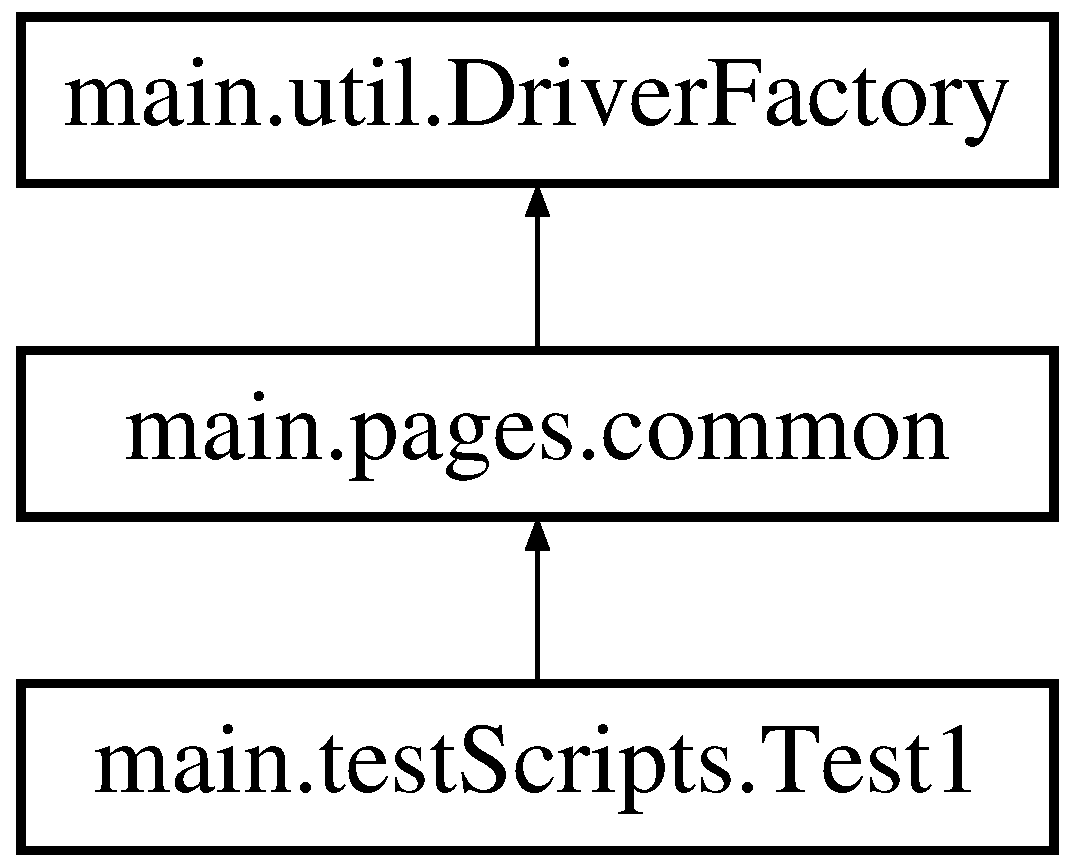
\includegraphics[height=3.000000cm]{classmain_1_1test_scripts_1_1_test1}
\end{center}
\end{figure}
\subsection*{Public Member Functions}
\begin{DoxyCompactItemize}
\item 
void \mbox{\hyperlink{classmain_1_1test_scripts_1_1_test1_a8dc6636009624d1b3d4dbbf804642e79}{before\+Test}} (String browser\+Type)
\item 
void \mbox{\hyperlink{classmain_1_1test_scripts_1_1_test1_a2c86a510c69dfa3237bcab629cc80a73}{verify\+App\+Title2}} ()
\item 
void \mbox{\hyperlink{classmain_1_1test_scripts_1_1_test1_aa27f8330d3cfc47141559c5799ed8139}{after\+Test}} ()
\end{DoxyCompactItemize}
\subsection*{Additional Inherited Members}


\subsection{Member Function Documentation}
\mbox{\Hypertarget{classmain_1_1test_scripts_1_1_test1_aa27f8330d3cfc47141559c5799ed8139}\label{classmain_1_1test_scripts_1_1_test1_aa27f8330d3cfc47141559c5799ed8139}} 
\index{main\+::test\+Scripts\+::\+Test1@{main\+::test\+Scripts\+::\+Test1}!after\+Test@{after\+Test}}
\index{after\+Test@{after\+Test}!main\+::test\+Scripts\+::\+Test1@{main\+::test\+Scripts\+::\+Test1}}
\subsubsection{\texorpdfstring{after\+Test()}{afterTest()}}
{\footnotesize\ttfamily void main.\+test\+Scripts.\+Test1.\+after\+Test (\begin{DoxyParamCaption}{ }\end{DoxyParamCaption})}

A  method to close the driver.. \begin{DoxyReturn}{Returns}
void 
\end{DoxyReturn}
\mbox{\Hypertarget{classmain_1_1test_scripts_1_1_test1_a8dc6636009624d1b3d4dbbf804642e79}\label{classmain_1_1test_scripts_1_1_test1_a8dc6636009624d1b3d4dbbf804642e79}} 
\index{main\+::test\+Scripts\+::\+Test1@{main\+::test\+Scripts\+::\+Test1}!before\+Test@{before\+Test}}
\index{before\+Test@{before\+Test}!main\+::test\+Scripts\+::\+Test1@{main\+::test\+Scripts\+::\+Test1}}
\subsubsection{\texorpdfstring{before\+Test()}{beforeTest()}}
{\footnotesize\ttfamily void main.\+test\+Scripts.\+Test1.\+before\+Test (\begin{DoxyParamCaption}\item[{String}]{browser\+Type }\end{DoxyParamCaption})}

A  method to initialize the driver \& other necessary instances of logger and assert.. \begin{DoxyReturn}{Returns}
void 
\end{DoxyReturn}
\mbox{\Hypertarget{classmain_1_1test_scripts_1_1_test1_a2c86a510c69dfa3237bcab629cc80a73}\label{classmain_1_1test_scripts_1_1_test1_a2c86a510c69dfa3237bcab629cc80a73}} 
\index{main\+::test\+Scripts\+::\+Test1@{main\+::test\+Scripts\+::\+Test1}!verify\+App\+Title2@{verify\+App\+Title2}}
\index{verify\+App\+Title2@{verify\+App\+Title2}!main\+::test\+Scripts\+::\+Test1@{main\+::test\+Scripts\+::\+Test1}}
\subsubsection{\texorpdfstring{verify\+App\+Title2()}{verifyAppTitle2()}}
{\footnotesize\ttfamily void main.\+test\+Scripts.\+Test1.\+verify\+App\+Title2 (\begin{DoxyParamCaption}{ }\end{DoxyParamCaption})}

A  methods to verify the title of the navigated page and all the necessary elements are available on the page. \begin{DoxyReturn}{Returns}
void 
\end{DoxyReturn}


The documentation for this class was generated from the following file\+:\begin{DoxyCompactItemize}
\item 
main/test\+Scripts/Test1.\+java\end{DoxyCompactItemize}

\hypertarget{classmain_1_1test_scripts_1_1_test2}{}\section{main.\+test\+Scripts.\+Test2 Class Reference}
\label{classmain_1_1test_scripts_1_1_test2}\index{main.\+test\+Scripts.\+Test2@{main.\+test\+Scripts.\+Test2}}
Inheritance diagram for main.\+test\+Scripts.\+Test2\+:\begin{figure}[H]
\begin{center}
\leavevmode
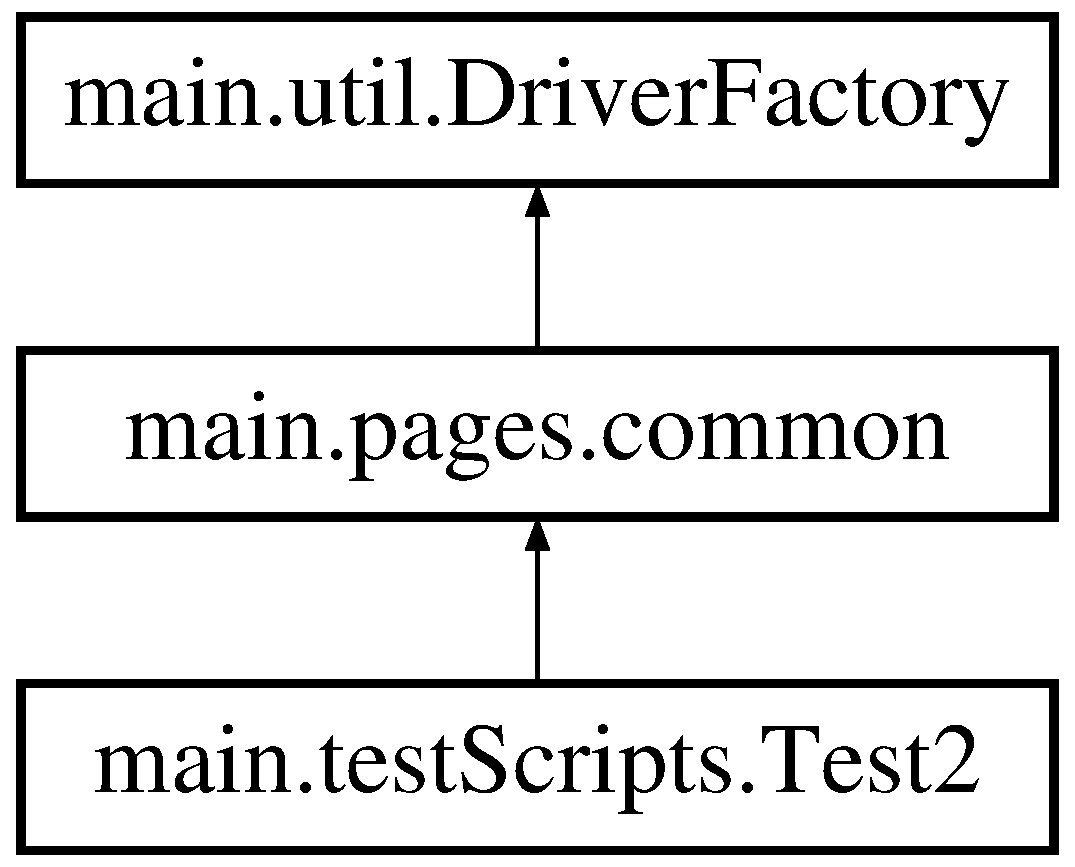
\includegraphics[height=3.000000cm]{classmain_1_1test_scripts_1_1_test2}
\end{center}
\end{figure}
\subsection*{Public Member Functions}
\begin{DoxyCompactItemize}
\item 
void \mbox{\hyperlink{classmain_1_1test_scripts_1_1_test2_add17ccdd24a07f4d61763a91b58071ff}{before\+Test}} (String browser\+Type)
\item 
void \mbox{\hyperlink{classmain_1_1test_scripts_1_1_test2_a6607310c15cc4d9f1ff7194d1cadf479}{search\+Textin\+Search\+Box}} (String City\+Name)
\item 
void \mbox{\hyperlink{classmain_1_1test_scripts_1_1_test2_a8cbf8c3569b59359240b66cc0bf45e08}{verify\+Searh\+Result\+Not\+Displayed}} ()
\item 
void \mbox{\hyperlink{classmain_1_1test_scripts_1_1_test2_aea588f2abffef056a18639409e0dddea}{after\+Test}} ()
\end{DoxyCompactItemize}
\subsection*{Additional Inherited Members}


\subsection{Member Function Documentation}
\mbox{\Hypertarget{classmain_1_1test_scripts_1_1_test2_aea588f2abffef056a18639409e0dddea}\label{classmain_1_1test_scripts_1_1_test2_aea588f2abffef056a18639409e0dddea}} 
\index{main\+::test\+Scripts\+::\+Test2@{main\+::test\+Scripts\+::\+Test2}!after\+Test@{after\+Test}}
\index{after\+Test@{after\+Test}!main\+::test\+Scripts\+::\+Test2@{main\+::test\+Scripts\+::\+Test2}}
\subsubsection{\texorpdfstring{after\+Test()}{afterTest()}}
{\footnotesize\ttfamily void main.\+test\+Scripts.\+Test2.\+after\+Test (\begin{DoxyParamCaption}{ }\end{DoxyParamCaption})}

A  method to close the driver.. \begin{DoxyReturn}{Returns}
void 
\end{DoxyReturn}
\mbox{\Hypertarget{classmain_1_1test_scripts_1_1_test2_add17ccdd24a07f4d61763a91b58071ff}\label{classmain_1_1test_scripts_1_1_test2_add17ccdd24a07f4d61763a91b58071ff}} 
\index{main\+::test\+Scripts\+::\+Test2@{main\+::test\+Scripts\+::\+Test2}!before\+Test@{before\+Test}}
\index{before\+Test@{before\+Test}!main\+::test\+Scripts\+::\+Test2@{main\+::test\+Scripts\+::\+Test2}}
\subsubsection{\texorpdfstring{before\+Test()}{beforeTest()}}
{\footnotesize\ttfamily void main.\+test\+Scripts.\+Test2.\+before\+Test (\begin{DoxyParamCaption}\item[{String}]{browser\+Type }\end{DoxyParamCaption})}

A  method to initialize the driver \& other necessary instances of logger and assert.. \begin{DoxyReturn}{Returns}
void 
\end{DoxyReturn}
\mbox{\Hypertarget{classmain_1_1test_scripts_1_1_test2_a6607310c15cc4d9f1ff7194d1cadf479}\label{classmain_1_1test_scripts_1_1_test2_a6607310c15cc4d9f1ff7194d1cadf479}} 
\index{main\+::test\+Scripts\+::\+Test2@{main\+::test\+Scripts\+::\+Test2}!search\+Textin\+Search\+Box@{search\+Textin\+Search\+Box}}
\index{search\+Textin\+Search\+Box@{search\+Textin\+Search\+Box}!main\+::test\+Scripts\+::\+Test2@{main\+::test\+Scripts\+::\+Test2}}
\subsubsection{\texorpdfstring{search\+Textin\+Search\+Box()}{searchTextinSearchBox()}}
{\footnotesize\ttfamily void main.\+test\+Scripts.\+Test2.\+search\+Textin\+Search\+Box (\begin{DoxyParamCaption}\item[{String}]{City\+Name }\end{DoxyParamCaption})}

A  methods to Verify the user is able to search using search box 
\begin{DoxyParams}{Parameters}
{\em City\+Name} & as a search text \\
\hline
\end{DoxyParams}
\begin{DoxyReturn}{Returns}
void 
\end{DoxyReturn}
\mbox{\Hypertarget{classmain_1_1test_scripts_1_1_test2_a8cbf8c3569b59359240b66cc0bf45e08}\label{classmain_1_1test_scripts_1_1_test2_a8cbf8c3569b59359240b66cc0bf45e08}} 
\index{main\+::test\+Scripts\+::\+Test2@{main\+::test\+Scripts\+::\+Test2}!verify\+Searh\+Result\+Not\+Displayed@{verify\+Searh\+Result\+Not\+Displayed}}
\index{verify\+Searh\+Result\+Not\+Displayed@{verify\+Searh\+Result\+Not\+Displayed}!main\+::test\+Scripts\+::\+Test2@{main\+::test\+Scripts\+::\+Test2}}
\subsubsection{\texorpdfstring{verify\+Searh\+Result\+Not\+Displayed()}{verifySearhResultNotDisplayed()}}
{\footnotesize\ttfamily void main.\+test\+Scripts.\+Test2.\+verify\+Searh\+Result\+Not\+Displayed (\begin{DoxyParamCaption}{ }\end{DoxyParamCaption})}

A  methods to Verify that the results are not displyed if user is given a invalid city name/arbitory data as a search \begin{DoxyReturn}{Returns}
void 
\end{DoxyReturn}


The documentation for this class was generated from the following file\+:\begin{DoxyCompactItemize}
\item 
main/test\+Scripts/Test2.\+java\end{DoxyCompactItemize}

\hypertarget{classmain_1_1test_scripts_1_1_test3}{}\section{main.\+test\+Scripts.\+Test3 Class Reference}
\label{classmain_1_1test_scripts_1_1_test3}\index{main.\+test\+Scripts.\+Test3@{main.\+test\+Scripts.\+Test3}}
Inheritance diagram for main.\+test\+Scripts.\+Test3\+:\begin{figure}[H]
\begin{center}
\leavevmode
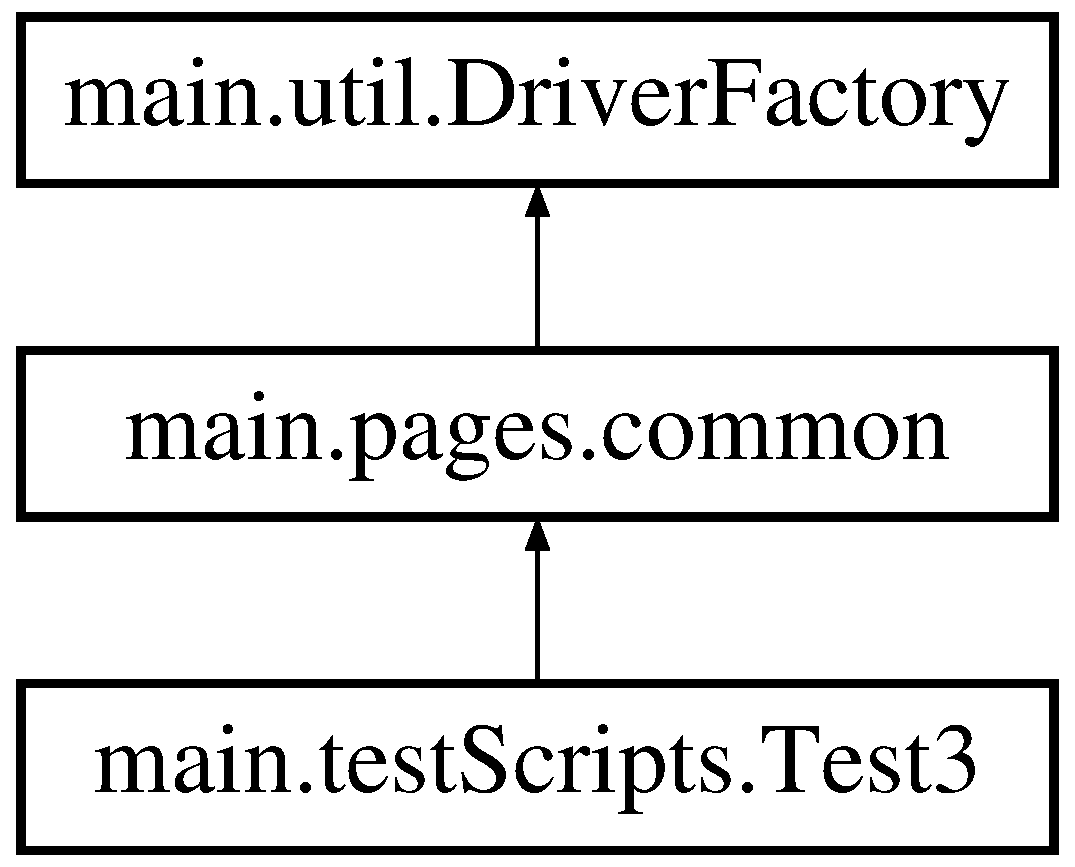
\includegraphics[height=3.000000cm]{classmain_1_1test_scripts_1_1_test3}
\end{center}
\end{figure}
\subsection*{Public Member Functions}
\begin{DoxyCompactItemize}
\item 
void \mbox{\hyperlink{classmain_1_1test_scripts_1_1_test3_a6def60a96025e336f8fa0d48c7de9707}{before\+Test}} (String browser\+Type)
\item 
void \mbox{\hyperlink{classmain_1_1test_scripts_1_1_test3_a7d7770a67e1c5d3b4412342457a039f6}{search\+Textin\+Search\+Box}} ()
\item 
void \mbox{\hyperlink{classmain_1_1test_scripts_1_1_test3_a1901c542d53d9249498e84984659df88}{verify\+Searh\+Result\+Displayed\+Sucessfully}} (String City\+Name)
\item 
void \mbox{\hyperlink{classmain_1_1test_scripts_1_1_test3_abacb83e061539da4aa9500d9ab76a98f}{after\+Test}} ()
\end{DoxyCompactItemize}
\subsection*{Additional Inherited Members}


\subsection{Member Function Documentation}
\mbox{\Hypertarget{classmain_1_1test_scripts_1_1_test3_abacb83e061539da4aa9500d9ab76a98f}\label{classmain_1_1test_scripts_1_1_test3_abacb83e061539da4aa9500d9ab76a98f}} 
\index{main\+::test\+Scripts\+::\+Test3@{main\+::test\+Scripts\+::\+Test3}!after\+Test@{after\+Test}}
\index{after\+Test@{after\+Test}!main\+::test\+Scripts\+::\+Test3@{main\+::test\+Scripts\+::\+Test3}}
\subsubsection{\texorpdfstring{after\+Test()}{afterTest()}}
{\footnotesize\ttfamily void main.\+test\+Scripts.\+Test3.\+after\+Test (\begin{DoxyParamCaption}{ }\end{DoxyParamCaption})}

A  method to close the driver.. \begin{DoxyReturn}{Returns}
void 
\end{DoxyReturn}
\mbox{\Hypertarget{classmain_1_1test_scripts_1_1_test3_a6def60a96025e336f8fa0d48c7de9707}\label{classmain_1_1test_scripts_1_1_test3_a6def60a96025e336f8fa0d48c7de9707}} 
\index{main\+::test\+Scripts\+::\+Test3@{main\+::test\+Scripts\+::\+Test3}!before\+Test@{before\+Test}}
\index{before\+Test@{before\+Test}!main\+::test\+Scripts\+::\+Test3@{main\+::test\+Scripts\+::\+Test3}}
\subsubsection{\texorpdfstring{before\+Test()}{beforeTest()}}
{\footnotesize\ttfamily void main.\+test\+Scripts.\+Test3.\+before\+Test (\begin{DoxyParamCaption}\item[{String}]{browser\+Type }\end{DoxyParamCaption})}

A  method to initialize the driver \& other necessary instances of logger and assert.. \begin{DoxyReturn}{Returns}
void 
\end{DoxyReturn}
\mbox{\Hypertarget{classmain_1_1test_scripts_1_1_test3_a7d7770a67e1c5d3b4412342457a039f6}\label{classmain_1_1test_scripts_1_1_test3_a7d7770a67e1c5d3b4412342457a039f6}} 
\index{main\+::test\+Scripts\+::\+Test3@{main\+::test\+Scripts\+::\+Test3}!search\+Textin\+Search\+Box@{search\+Textin\+Search\+Box}}
\index{search\+Textin\+Search\+Box@{search\+Textin\+Search\+Box}!main\+::test\+Scripts\+::\+Test3@{main\+::test\+Scripts\+::\+Test3}}
\subsubsection{\texorpdfstring{search\+Textin\+Search\+Box()}{searchTextinSearchBox()}}
{\footnotesize\ttfamily void main.\+test\+Scripts.\+Test3.\+search\+Textin\+Search\+Box (\begin{DoxyParamCaption}{ }\end{DoxyParamCaption})}

A  methods to Verify that the user is able to search using search box \begin{DoxyReturn}{Returns}
void 
\end{DoxyReturn}
\mbox{\Hypertarget{classmain_1_1test_scripts_1_1_test3_a1901c542d53d9249498e84984659df88}\label{classmain_1_1test_scripts_1_1_test3_a1901c542d53d9249498e84984659df88}} 
\index{main\+::test\+Scripts\+::\+Test3@{main\+::test\+Scripts\+::\+Test3}!verify\+Searh\+Result\+Displayed\+Sucessfully@{verify\+Searh\+Result\+Displayed\+Sucessfully}}
\index{verify\+Searh\+Result\+Displayed\+Sucessfully@{verify\+Searh\+Result\+Displayed\+Sucessfully}!main\+::test\+Scripts\+::\+Test3@{main\+::test\+Scripts\+::\+Test3}}
\subsubsection{\texorpdfstring{verify\+Searh\+Result\+Displayed\+Sucessfully()}{verifySearhResultDisplayedSucessfully()}}
{\footnotesize\ttfamily void main.\+test\+Scripts.\+Test3.\+verify\+Searh\+Result\+Displayed\+Sucessfully (\begin{DoxyParamCaption}\item[{String}]{City\+Name }\end{DoxyParamCaption})}

A  methods to Verify that the results are displyed if user is given a valid city name as a search text 
\begin{DoxyParams}{Parameters}
{\em City} & name as a search text \\
\hline
\end{DoxyParams}
\begin{DoxyReturn}{Returns}
void 
\end{DoxyReturn}


The documentation for this class was generated from the following file\+:\begin{DoxyCompactItemize}
\item 
main/test\+Scripts/Test3.\+java\end{DoxyCompactItemize}

\hypertarget{classmain_1_1test_scripts_1_1_test4}{}\section{main.\+test\+Scripts.\+Test4 Class Reference}
\label{classmain_1_1test_scripts_1_1_test4}\index{main.\+test\+Scripts.\+Test4@{main.\+test\+Scripts.\+Test4}}
Inheritance diagram for main.\+test\+Scripts.\+Test4\+:\begin{figure}[H]
\begin{center}
\leavevmode
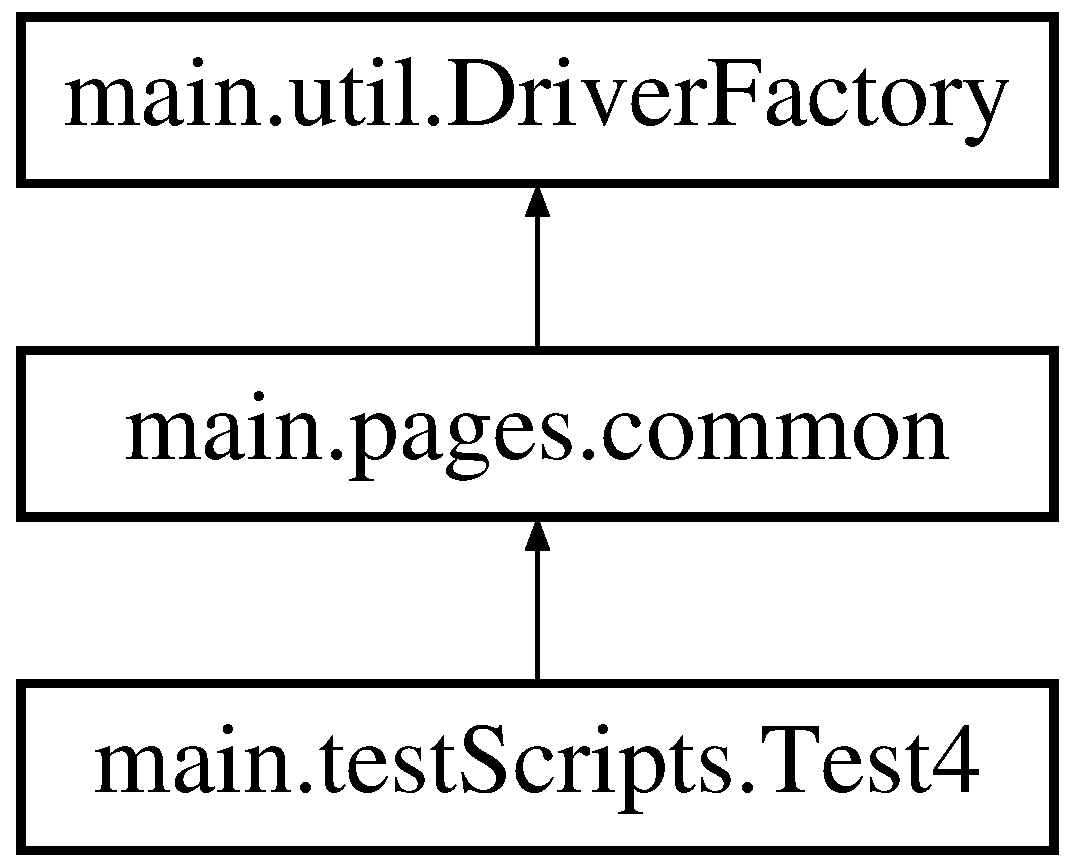
\includegraphics[height=3.000000cm]{classmain_1_1test_scripts_1_1_test4}
\end{center}
\end{figure}
\subsection*{Public Member Functions}
\begin{DoxyCompactItemize}
\item 
void \mbox{\hyperlink{classmain_1_1test_scripts_1_1_test4_a05a50b74977f548b1bfef2a49a114a3a}{before\+Test}} (String browser\+Type)
\item 
void \mbox{\hyperlink{classmain_1_1test_scripts_1_1_test4_ab572b49f4fa2052ad6428c1b0563c9ea}{valid\+Linls\+On\+Page}} ()
\item 
void \mbox{\hyperlink{classmain_1_1test_scripts_1_1_test4_a9a4eac7690ddbe8e60a940e54f7775b7}{after\+Test}} ()
\end{DoxyCompactItemize}
\subsection*{Additional Inherited Members}


\subsection{Member Function Documentation}
\mbox{\Hypertarget{classmain_1_1test_scripts_1_1_test4_a9a4eac7690ddbe8e60a940e54f7775b7}\label{classmain_1_1test_scripts_1_1_test4_a9a4eac7690ddbe8e60a940e54f7775b7}} 
\index{main\+::test\+Scripts\+::\+Test4@{main\+::test\+Scripts\+::\+Test4}!after\+Test@{after\+Test}}
\index{after\+Test@{after\+Test}!main\+::test\+Scripts\+::\+Test4@{main\+::test\+Scripts\+::\+Test4}}
\subsubsection{\texorpdfstring{after\+Test()}{afterTest()}}
{\footnotesize\ttfamily void main.\+test\+Scripts.\+Test4.\+after\+Test (\begin{DoxyParamCaption}{ }\end{DoxyParamCaption})}

A  method to close the driver.. \begin{DoxyReturn}{Returns}
void 
\end{DoxyReturn}
\mbox{\Hypertarget{classmain_1_1test_scripts_1_1_test4_a05a50b74977f548b1bfef2a49a114a3a}\label{classmain_1_1test_scripts_1_1_test4_a05a50b74977f548b1bfef2a49a114a3a}} 
\index{main\+::test\+Scripts\+::\+Test4@{main\+::test\+Scripts\+::\+Test4}!before\+Test@{before\+Test}}
\index{before\+Test@{before\+Test}!main\+::test\+Scripts\+::\+Test4@{main\+::test\+Scripts\+::\+Test4}}
\subsubsection{\texorpdfstring{before\+Test()}{beforeTest()}}
{\footnotesize\ttfamily void main.\+test\+Scripts.\+Test4.\+before\+Test (\begin{DoxyParamCaption}\item[{String}]{browser\+Type }\end{DoxyParamCaption})}

A  method to initialize the driver \& other necessary instances of logger and assert.. \begin{DoxyReturn}{Returns}
void 
\end{DoxyReturn}
\mbox{\Hypertarget{classmain_1_1test_scripts_1_1_test4_ab572b49f4fa2052ad6428c1b0563c9ea}\label{classmain_1_1test_scripts_1_1_test4_ab572b49f4fa2052ad6428c1b0563c9ea}} 
\index{main\+::test\+Scripts\+::\+Test4@{main\+::test\+Scripts\+::\+Test4}!valid\+Linls\+On\+Page@{valid\+Linls\+On\+Page}}
\index{valid\+Linls\+On\+Page@{valid\+Linls\+On\+Page}!main\+::test\+Scripts\+::\+Test4@{main\+::test\+Scripts\+::\+Test4}}
\subsubsection{\texorpdfstring{valid\+Linls\+On\+Page()}{validLinlsOnPage()}}
{\footnotesize\ttfamily void main.\+test\+Scripts.\+Test4.\+valid\+Linls\+On\+Page (\begin{DoxyParamCaption}{ }\end{DoxyParamCaption})}

A  methods to Verify that all the links available on Home page are valid links \begin{DoxyReturn}{Returns}
void 
\end{DoxyReturn}


The documentation for this class was generated from the following file\+:\begin{DoxyCompactItemize}
\item 
main/test\+Scripts/Test4.\+java\end{DoxyCompactItemize}

%--- End generated contents ---

% Index
\backmatter
\newpage
\phantomsection
\clearemptydoublepage
\addcontentsline{toc}{chapter}{Index}
\printindex

\end{document}
